\documentclass[12pt]{beamer}


\usetheme[progressbar=frametitle]{metropolis}
\usepackage{appendixnumberbeamer}

\usepackage{booktabs}
\usepackage[scale=2]{ccicons}

%\usepackage{pgfplots}
%\usepgfplotslibrary{dateplot}

\usepackage{xspace}
\newcommand{\themename}{\textbf{\textsc{metropolis}}\xspace}

%\setbeamertemplate{footline} % To remove the footer line in all slides uncomment this line
%\setbeamertemplate{footline}[page number] % To replace the footer line in all slides with a simple slide count uncomment this line

%\setbeamertemplate{navigation symbols}{} % To remove the navigation symbols from the bottom of all slides uncomment this line


\usepackage{graphicx} % Allows including images
\usepackage{grffile}
\usepackage{amsmath}
\usepackage{adjustbox} 
% have to have Mozilla's=Fira Sans} font and XeTeX installed to use full typography.

%----------------------------------------------------------------------------------------
%	TITLE PAGE
%----------------------------------------------------------------------------------------

\title{Collective Action or Exchange?: Framing International Cooperation in Alliance Politics}
\date{September 11, 2020}
\author{Joshua Alley}
\institute{University of Virginia}


\begin{document}

 \maketitle


%----------------------------------------------------------------------------------------
%	PRESENTATION SLIDES
%----------------------------------------------------------------------------------------

%------------------------------------------------
% Here's my point. 
 \begin{frame}[standout]

How do elite frames of allied military spending affect public support for cooperation in alliances? 

 \end{frame}
 

%------------------------------------------------

\begin{frame}{Why Should You Care?}

\begin{figure}[htbp]
		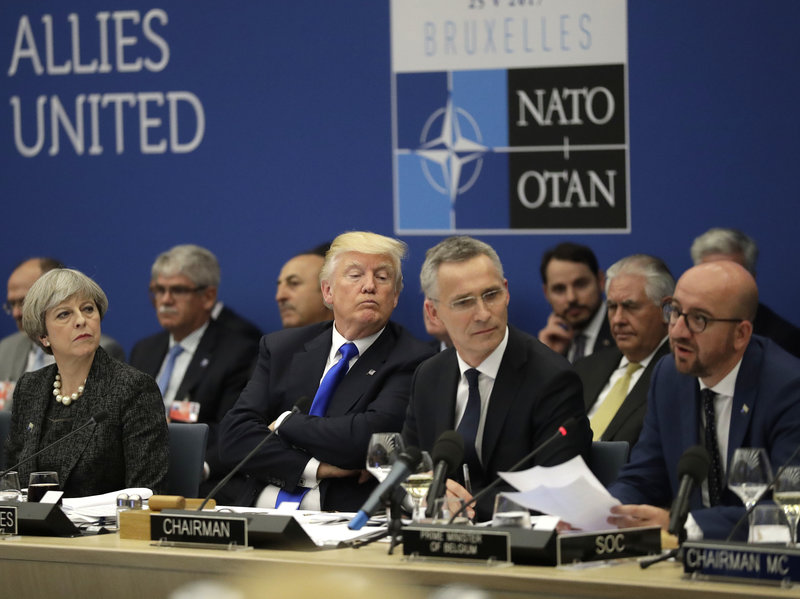
\includegraphics[width=0.95\textwidth]{trump-nato.jpg}
	\label{fig:trump-nato}
\end{figure}


\end{frame}

%------------------------------------------------

\begin{frame}{Outline}

\pause
\begin{enumerate}
\item Brief Argument Overview.
\pause
\item Experimental Design. 
\pause
\item Results from Mechanical Turk pretest. 
\end{enumerate}


\end{frame}
 

%------------------------------------------------

\section{Argument} 

%-----------------------------------------------

\begin{frame}{Two Frames of International Cooperation}

Rooted in academic theories/ideas:

\pause 
\begin{enumerate} 
\item \textbf{Collective Action}: Cooperate by contributing to some common/public good. 
\pause 
\item \textbf{Exchange}: Cooperate by trading different goods. 
\end{enumerate}


\end{frame} 

%-----------------------------------------------

\begin{frame}{Framing Spending by Alliance Members}

Foreign policy elites can use either general argument to frame/explain allied military spending. 

\pause 
\begin{enumerate} 
\item \textbf{Collective Action}: Free-riding and disproportionate contributions. 
\pause 
\item \textbf{Exchange}: Trading different foreign policy goods- security for influence. 
\end{enumerate}


\end{frame} 

%-----------------------------------------------

\begin{frame}{Predictions}

When applied to low allied military spending: 
\pause 
\begin{enumerate} 
\item \textbf{Collective Action}: Reduces support for cooperation: conditional cooperation and exploitation aversion. 
\pause 
\item \textbf{Exchange}: Greater support for cooperation: reciprocity. 
\end{enumerate}


\end{frame} 



%------------------------------------------------

\section{Experimental Design} 

%-----------------------------------------------

\begin{frame}{Emphasis}

Attitudes towards NATO in the United States. Randomly assign neutral, collective action or exchange vignette about NATO and military spending. 

\pause 
\begin{enumerate} 
\item Favorability towards NATO. 
\pause 
\item Support for withdrawal. 
\pause
\item Support for nonintervention. 
\end{enumerate}


\end{frame} 

%-----------------------------------------------

\begin{frame}{Vignettes}


\begin{enumerate}

\item \textbf{Neutral}: The United States has an important role in the North Atlantic Treaty Organization (NATO). NATO is a military alliance where members promise to support one another in war. According to an expert at the Council on Foreign Relations, a non-partisan think tank, some NATO members spend a smaller share of their resources on the military than the United States. 
\pause
\item \textbf{Collective Action}: adds \textit{because the United States provides a disproportionate share of security resources for the whole alliance.} 
\pause
\item \textbf{Exchange}: adds \textit{because they support US initiatives and goals in international politics in exchange for US protection.}
 
\end{enumerate} 

\end{frame} 


%-----------------------------------------------

\begin{frame}{Response Questions}


\begin{enumerate}

\item \textbf{Favorability}: 1-5 scale from Very Unfavorable to Very Favorable.  
\pause 
\item \textbf{Policy Response}:\textit{What should US leaders do, if anything, in response to allied defense spending?:} 
\begin{itemize}
\item Cooperate more with allies in defense planning.
\item Nothing. 
\item Give a verbal warning.
\item Impose economic sanctions.
\item Withdraw from the NATO alliance. 
\end{itemize} 
\pause 
\item \textbf{Intervention}: \textit{If Russia got into a serious military conflict with one of its neighboring countries that is our NATO ally, do you think the United States should or should not use military force to defend that country?}
 
\end{enumerate} 

\end{frame} 



%------------------------------------------------

\section{Pretest Results} 

%-----------------------------------------------


\begin{frame}{Favorability}

\begin{figure}[htbp]
	\centering
		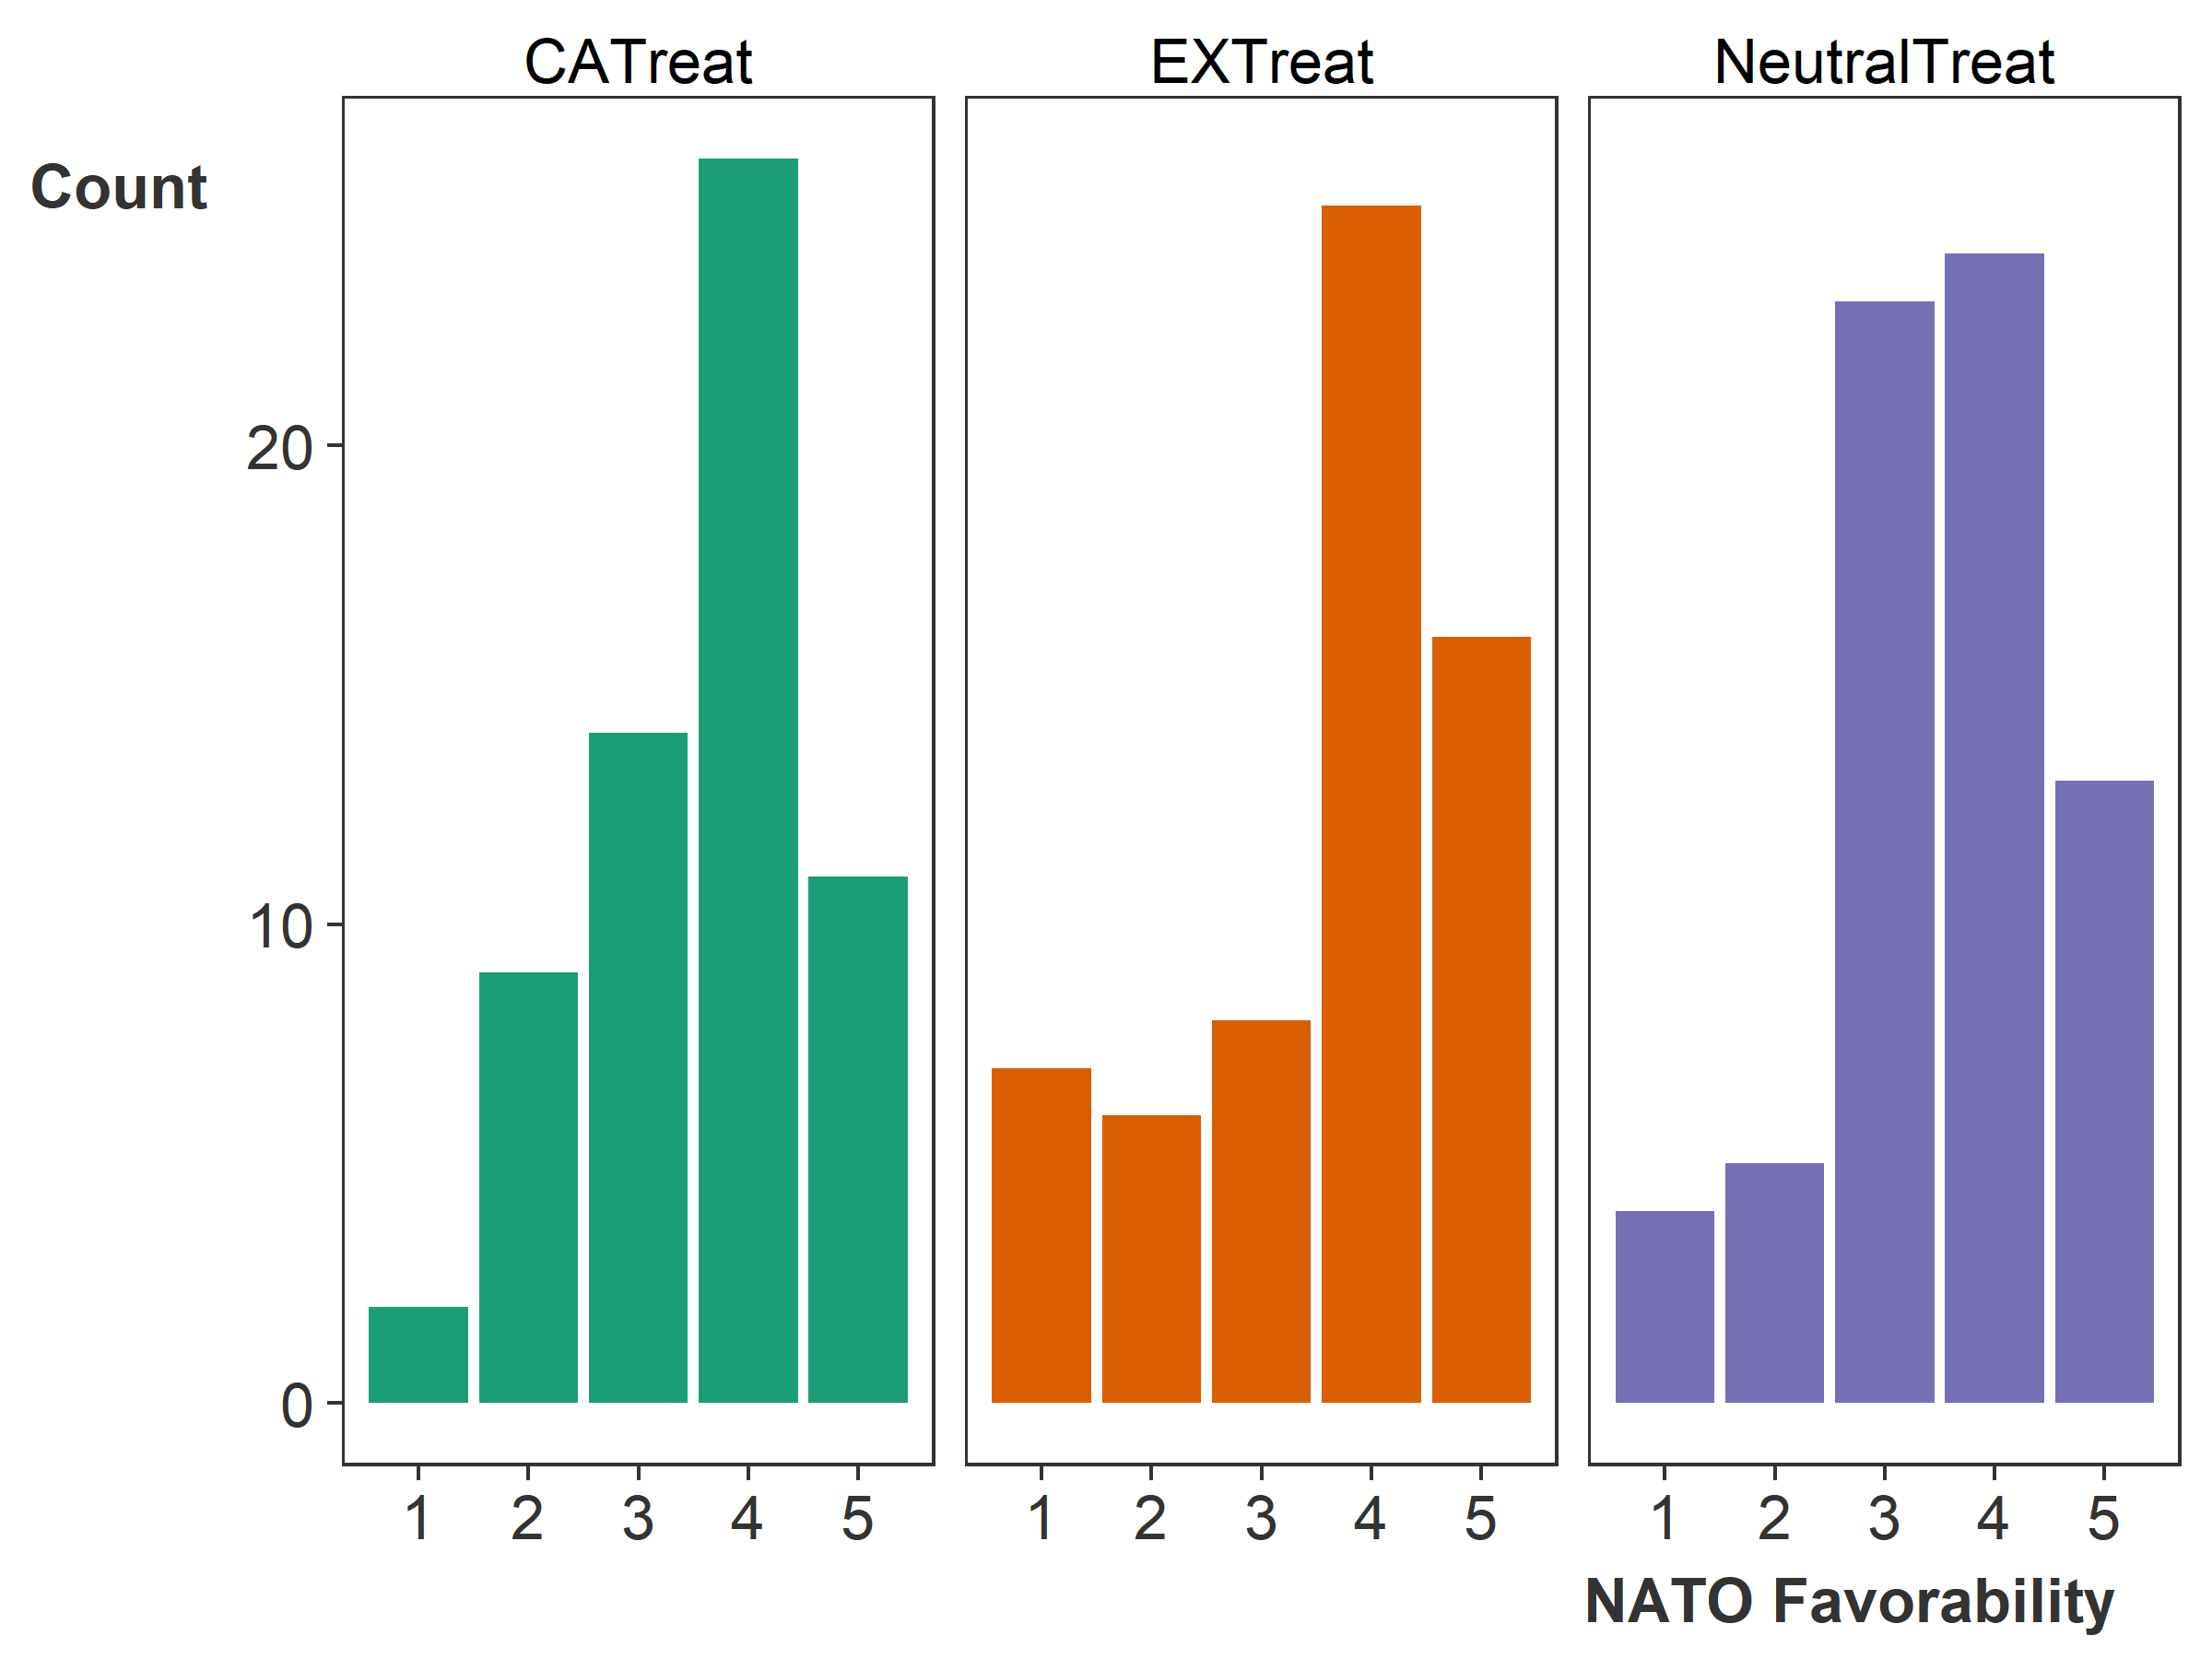
\includegraphics[width=0.95\textwidth]{raw-favor.png}
\end{figure}


\end{frame}

%-----------------------------------------------


\begin{frame}{Nonintervention}

\begin{figure}[htbp]
	\centering
		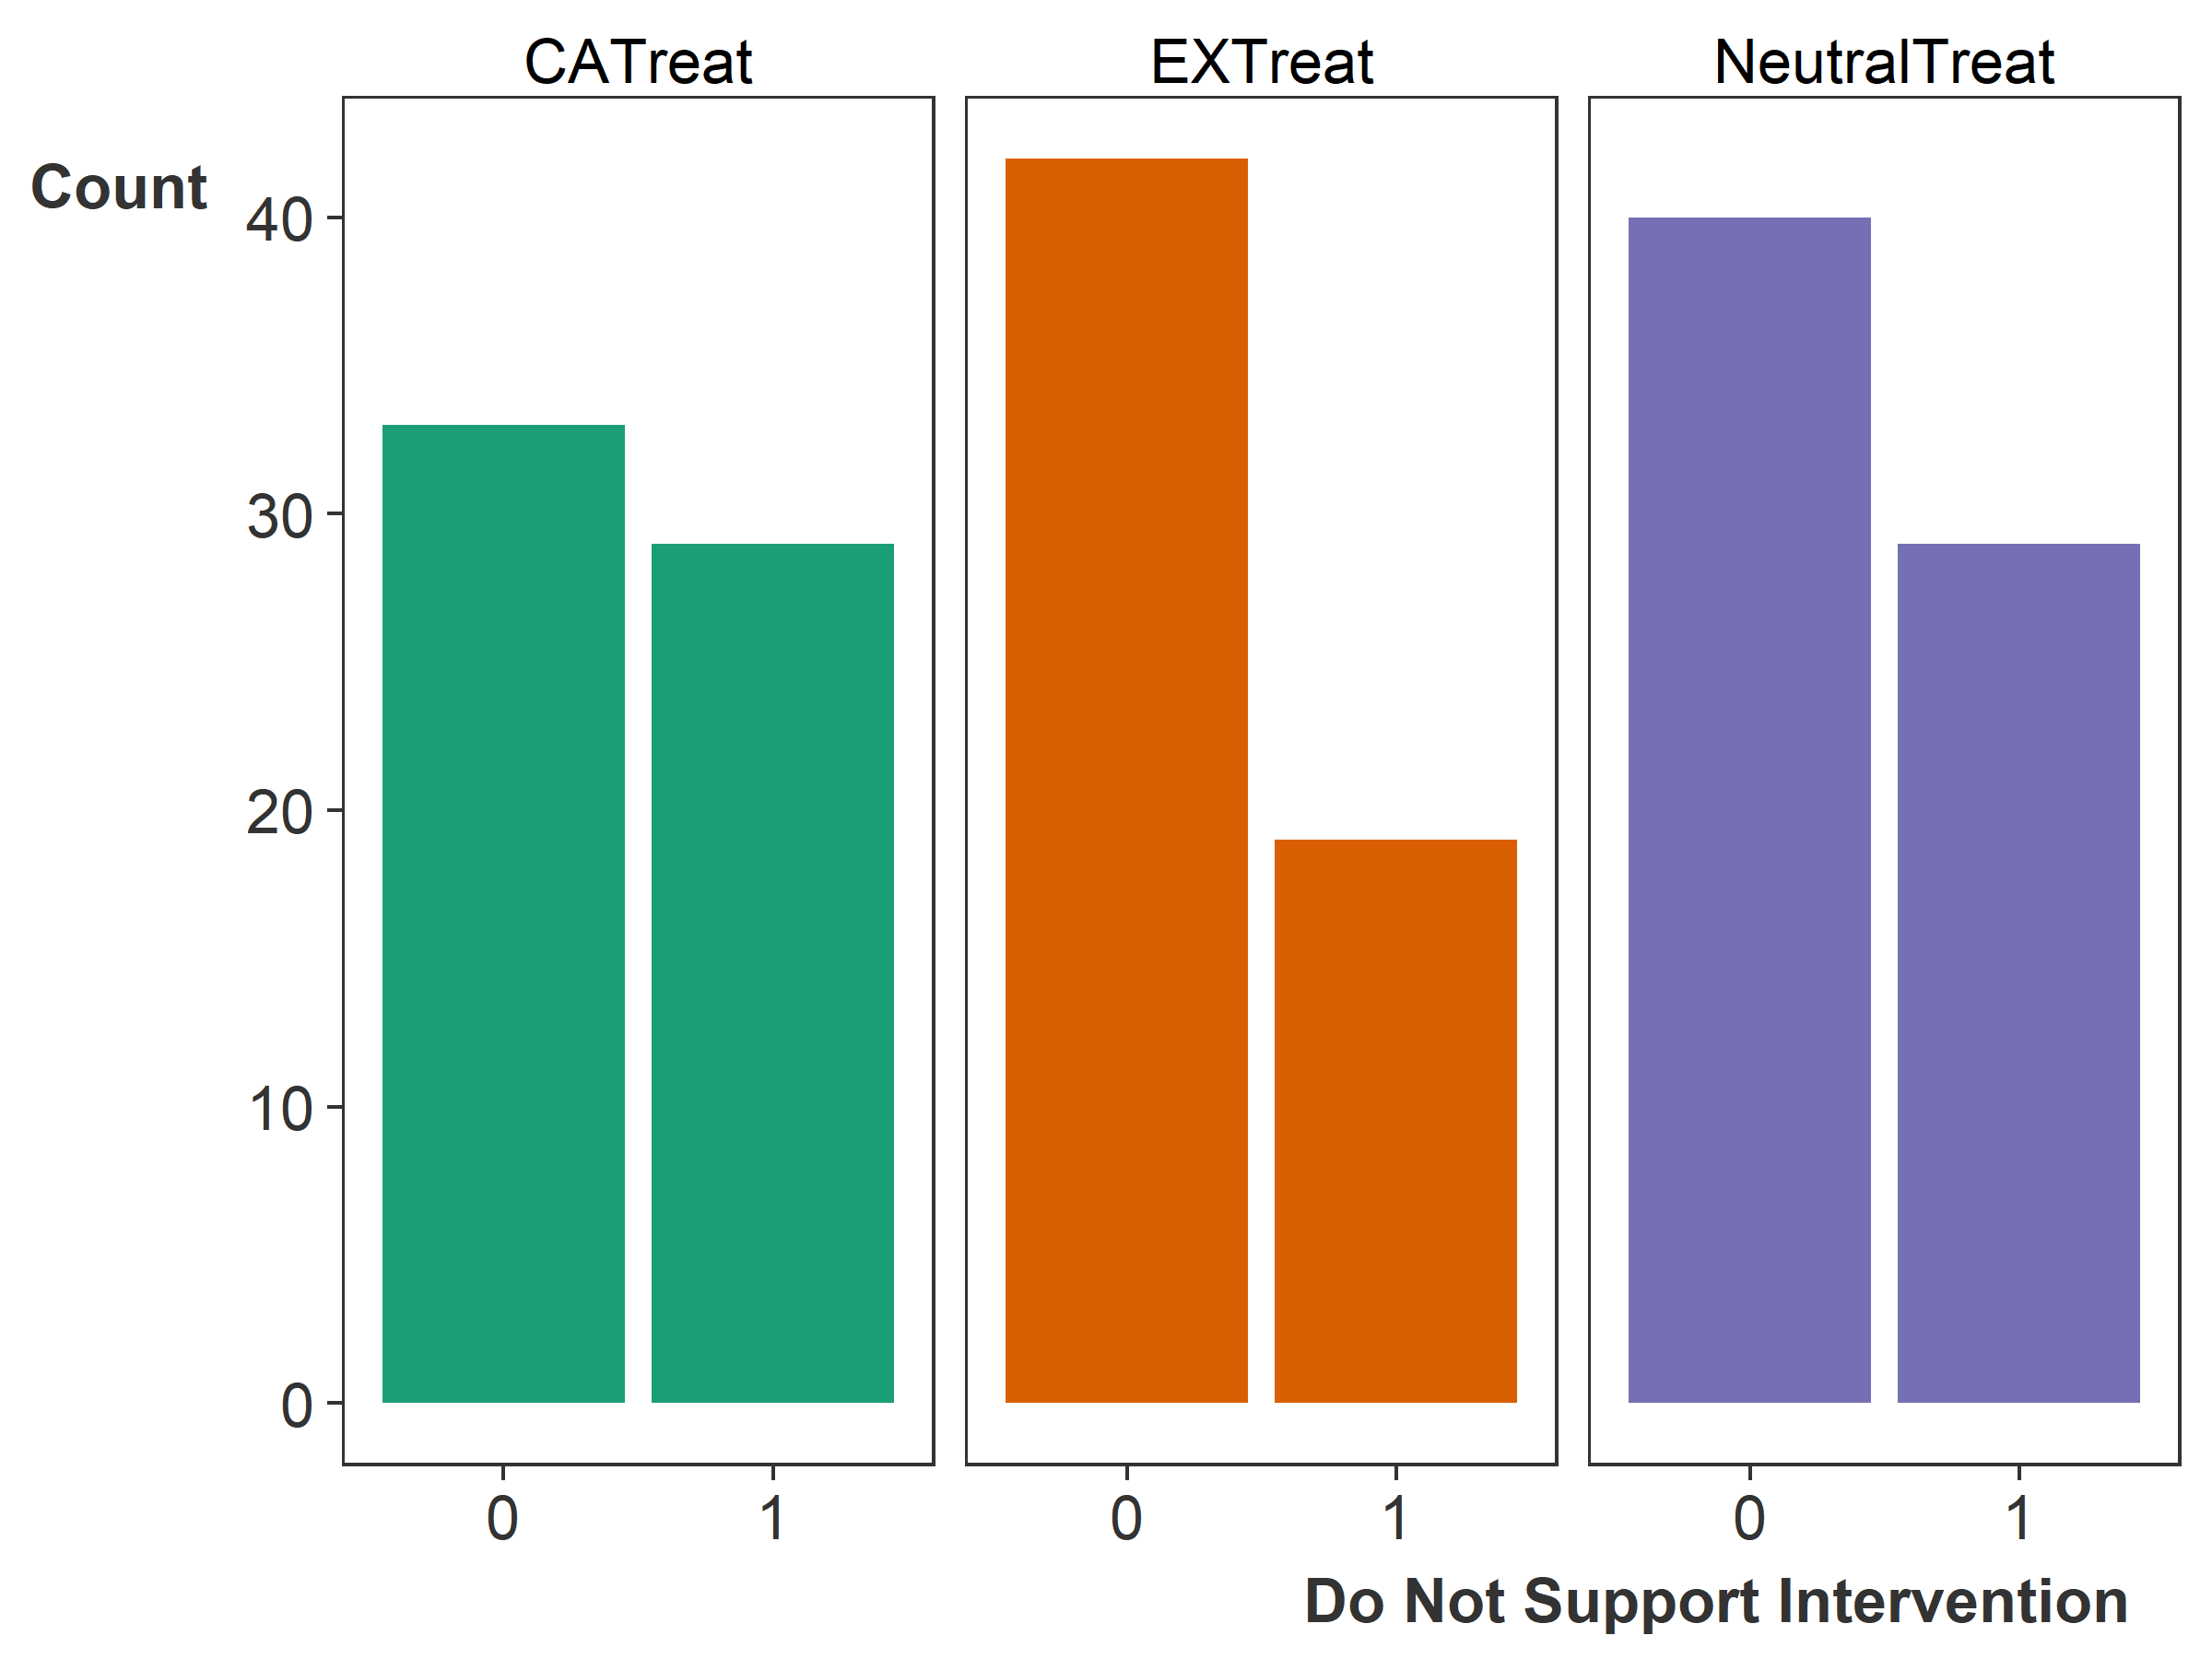
\includegraphics[width=0.95\textwidth]{raw-interv.png}
\end{figure}


\end{frame}

%-----------------------------------------------


\begin{frame}{Preferred Policy Response}

\begin{figure}[htbp]
	\centering
		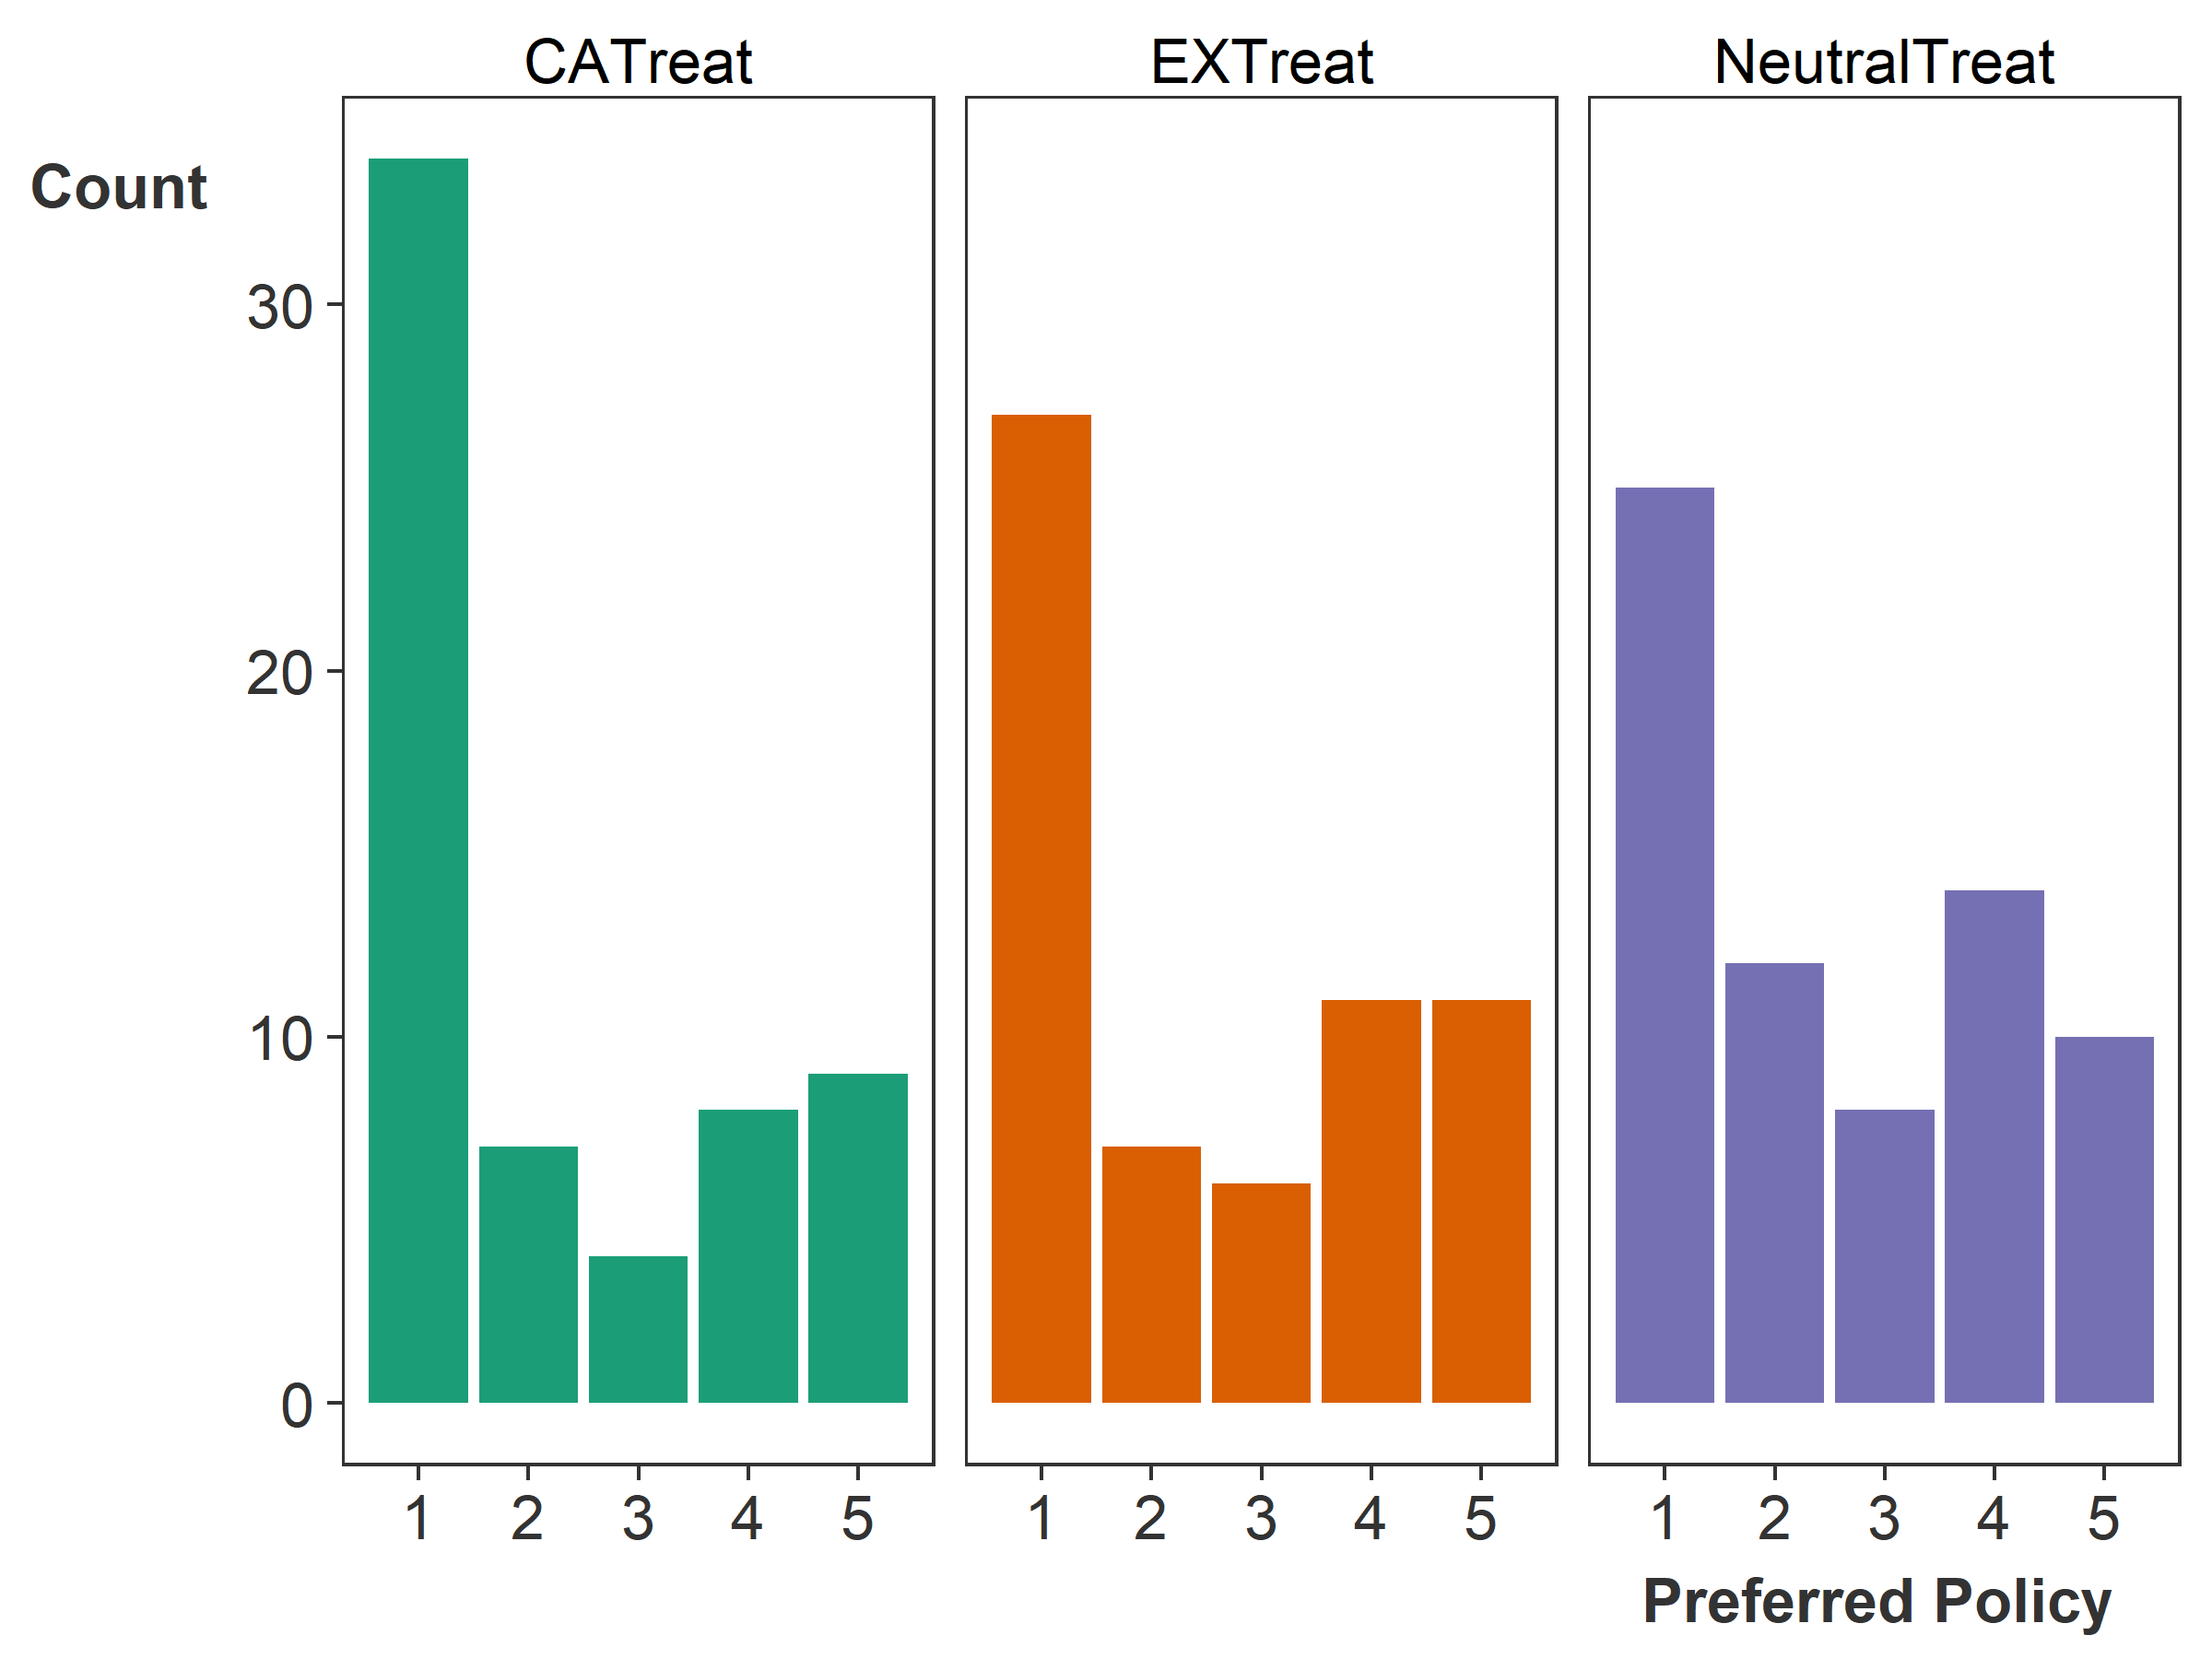
\includegraphics[width=0.95\textwidth]{raw-policy.png}
\end{figure}


\end{frame}

%-----------------------------------------------


\begin{frame}{Withdrawal}

\begin{figure}[htbp]
	\centering
		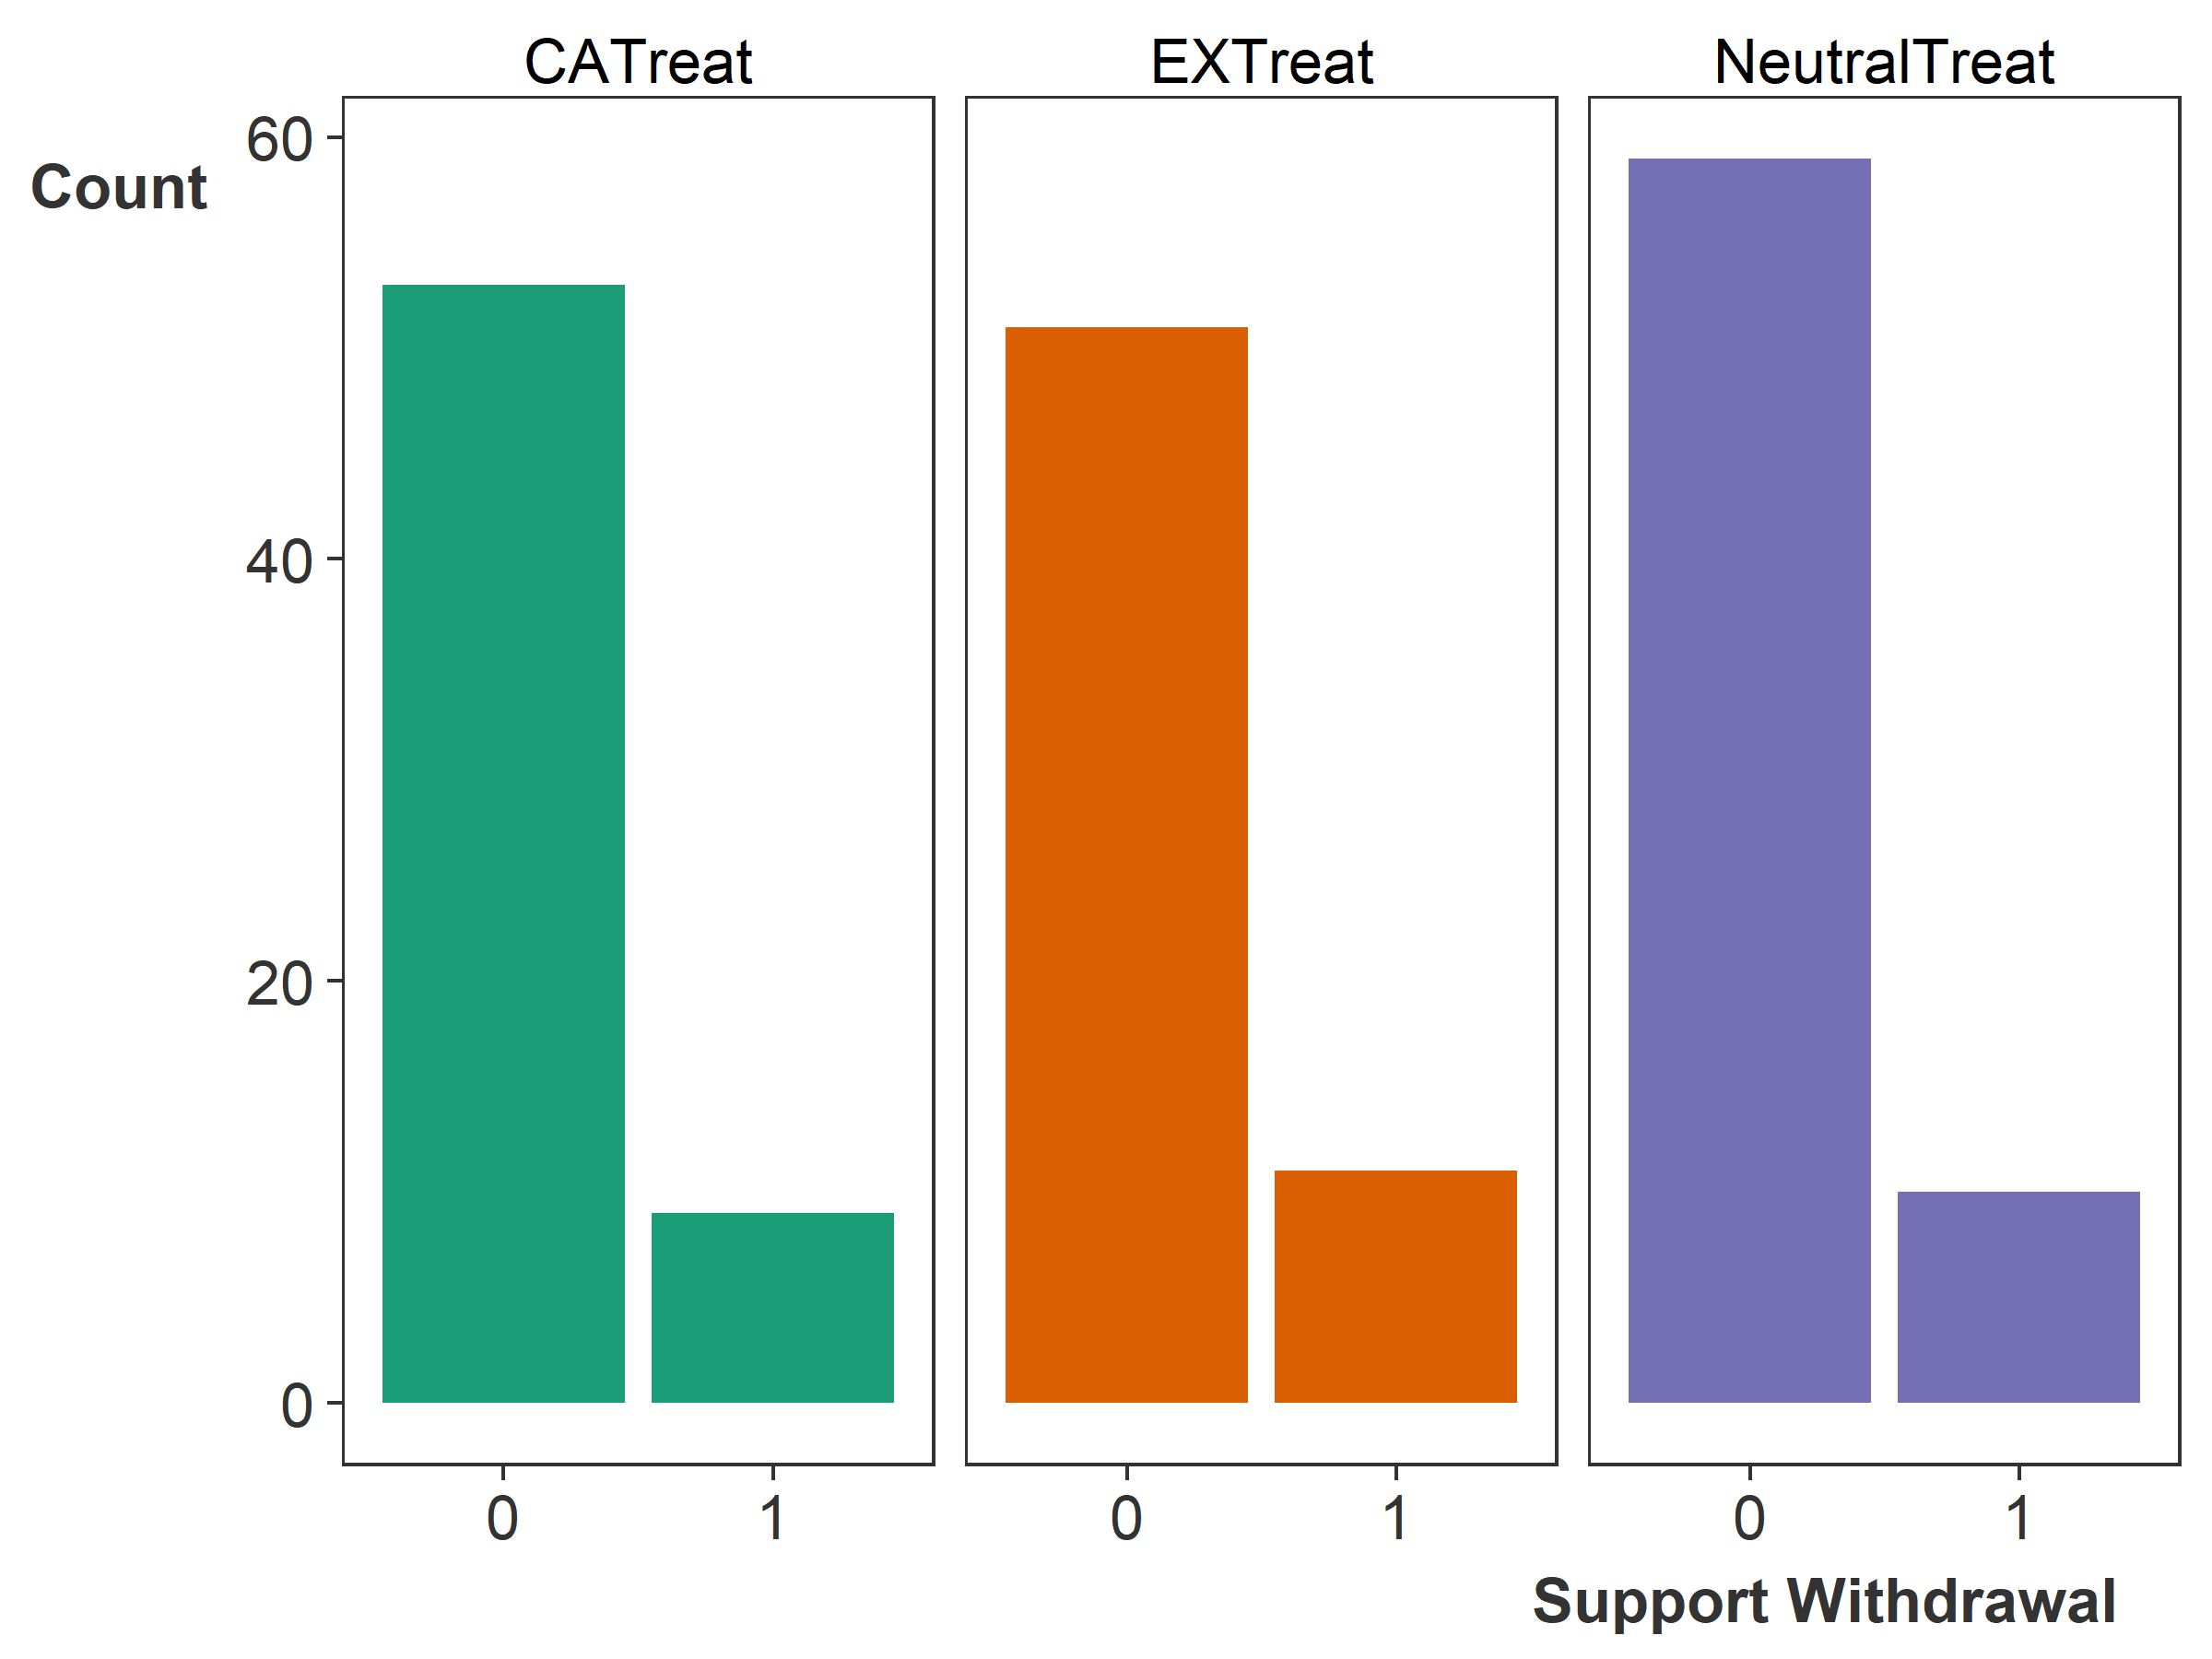
\includegraphics[width=0.95\textwidth]{raw-withdraw.png}
\end{figure}


\end{frame}


%-----------------------------------------------


\begin{frame}{Collective Action Treatment Effects}

\begin{figure}[htbp]
	\centering
		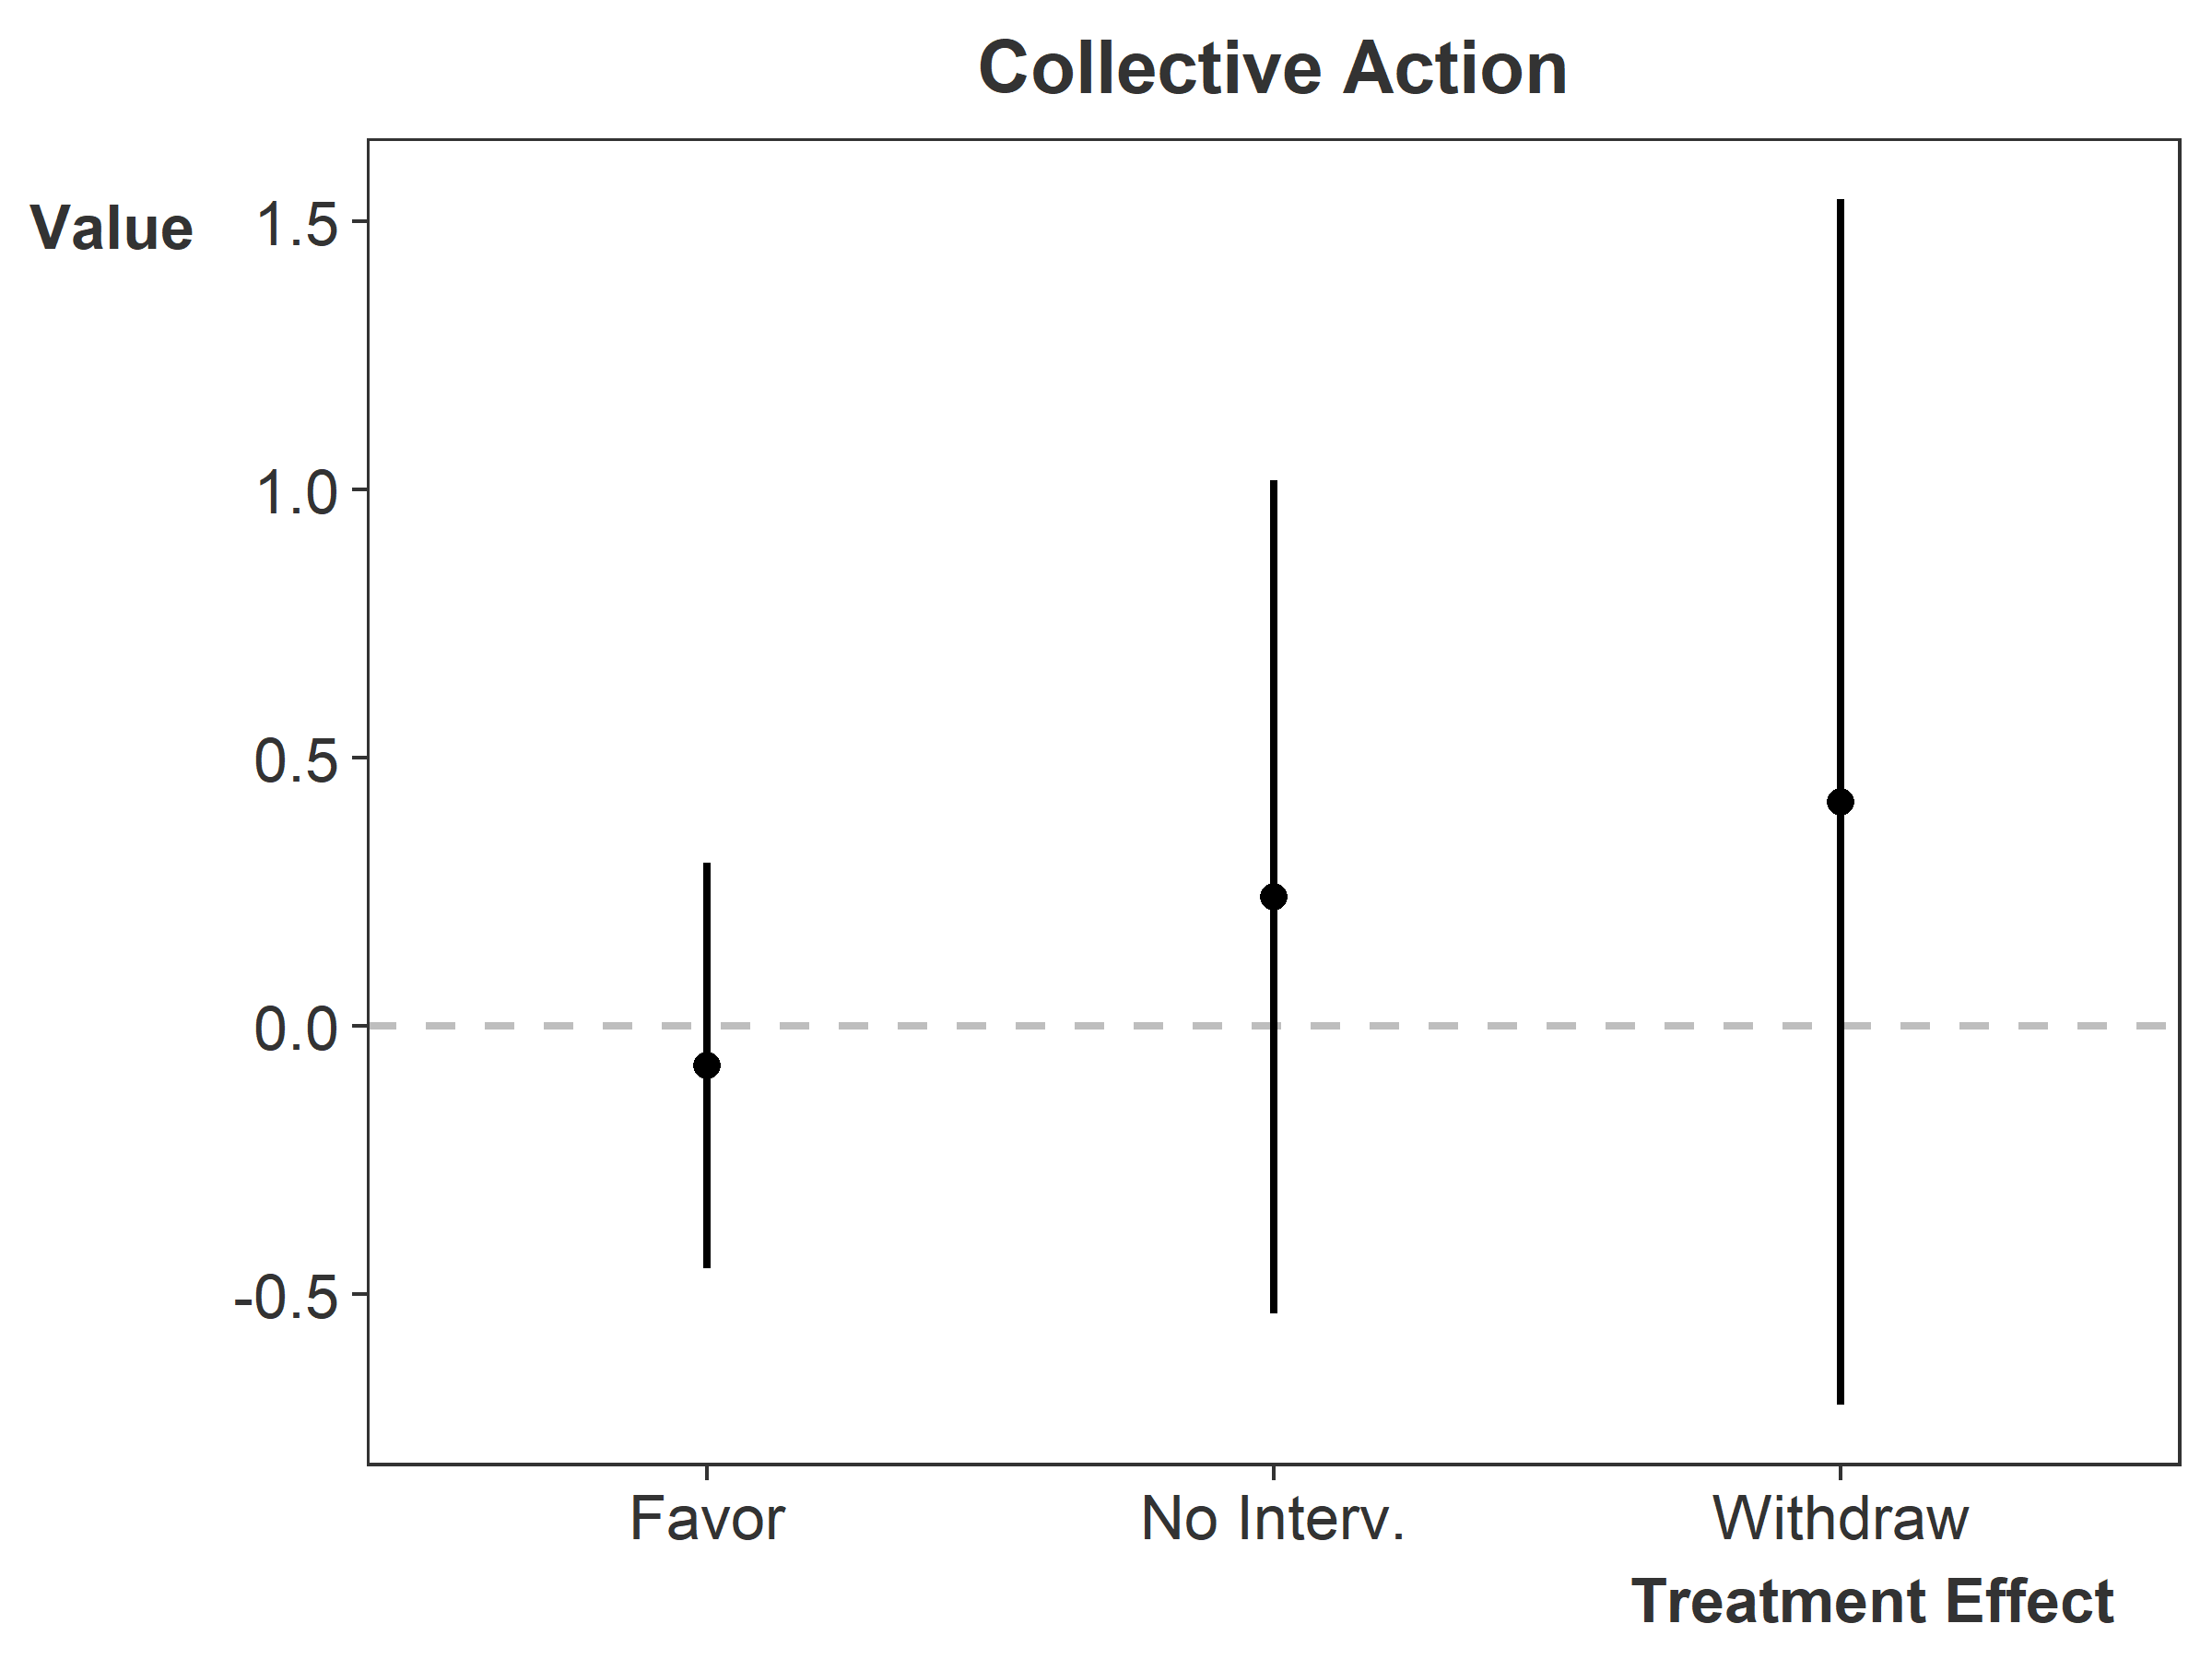
\includegraphics[width=0.95\textwidth]{ca-treat.png}
\end{figure}


\end{frame}

%-----------------------------------------------


\begin{frame}{Exchange Treatment Effects}

\begin{figure}[htbp]
	\centering
		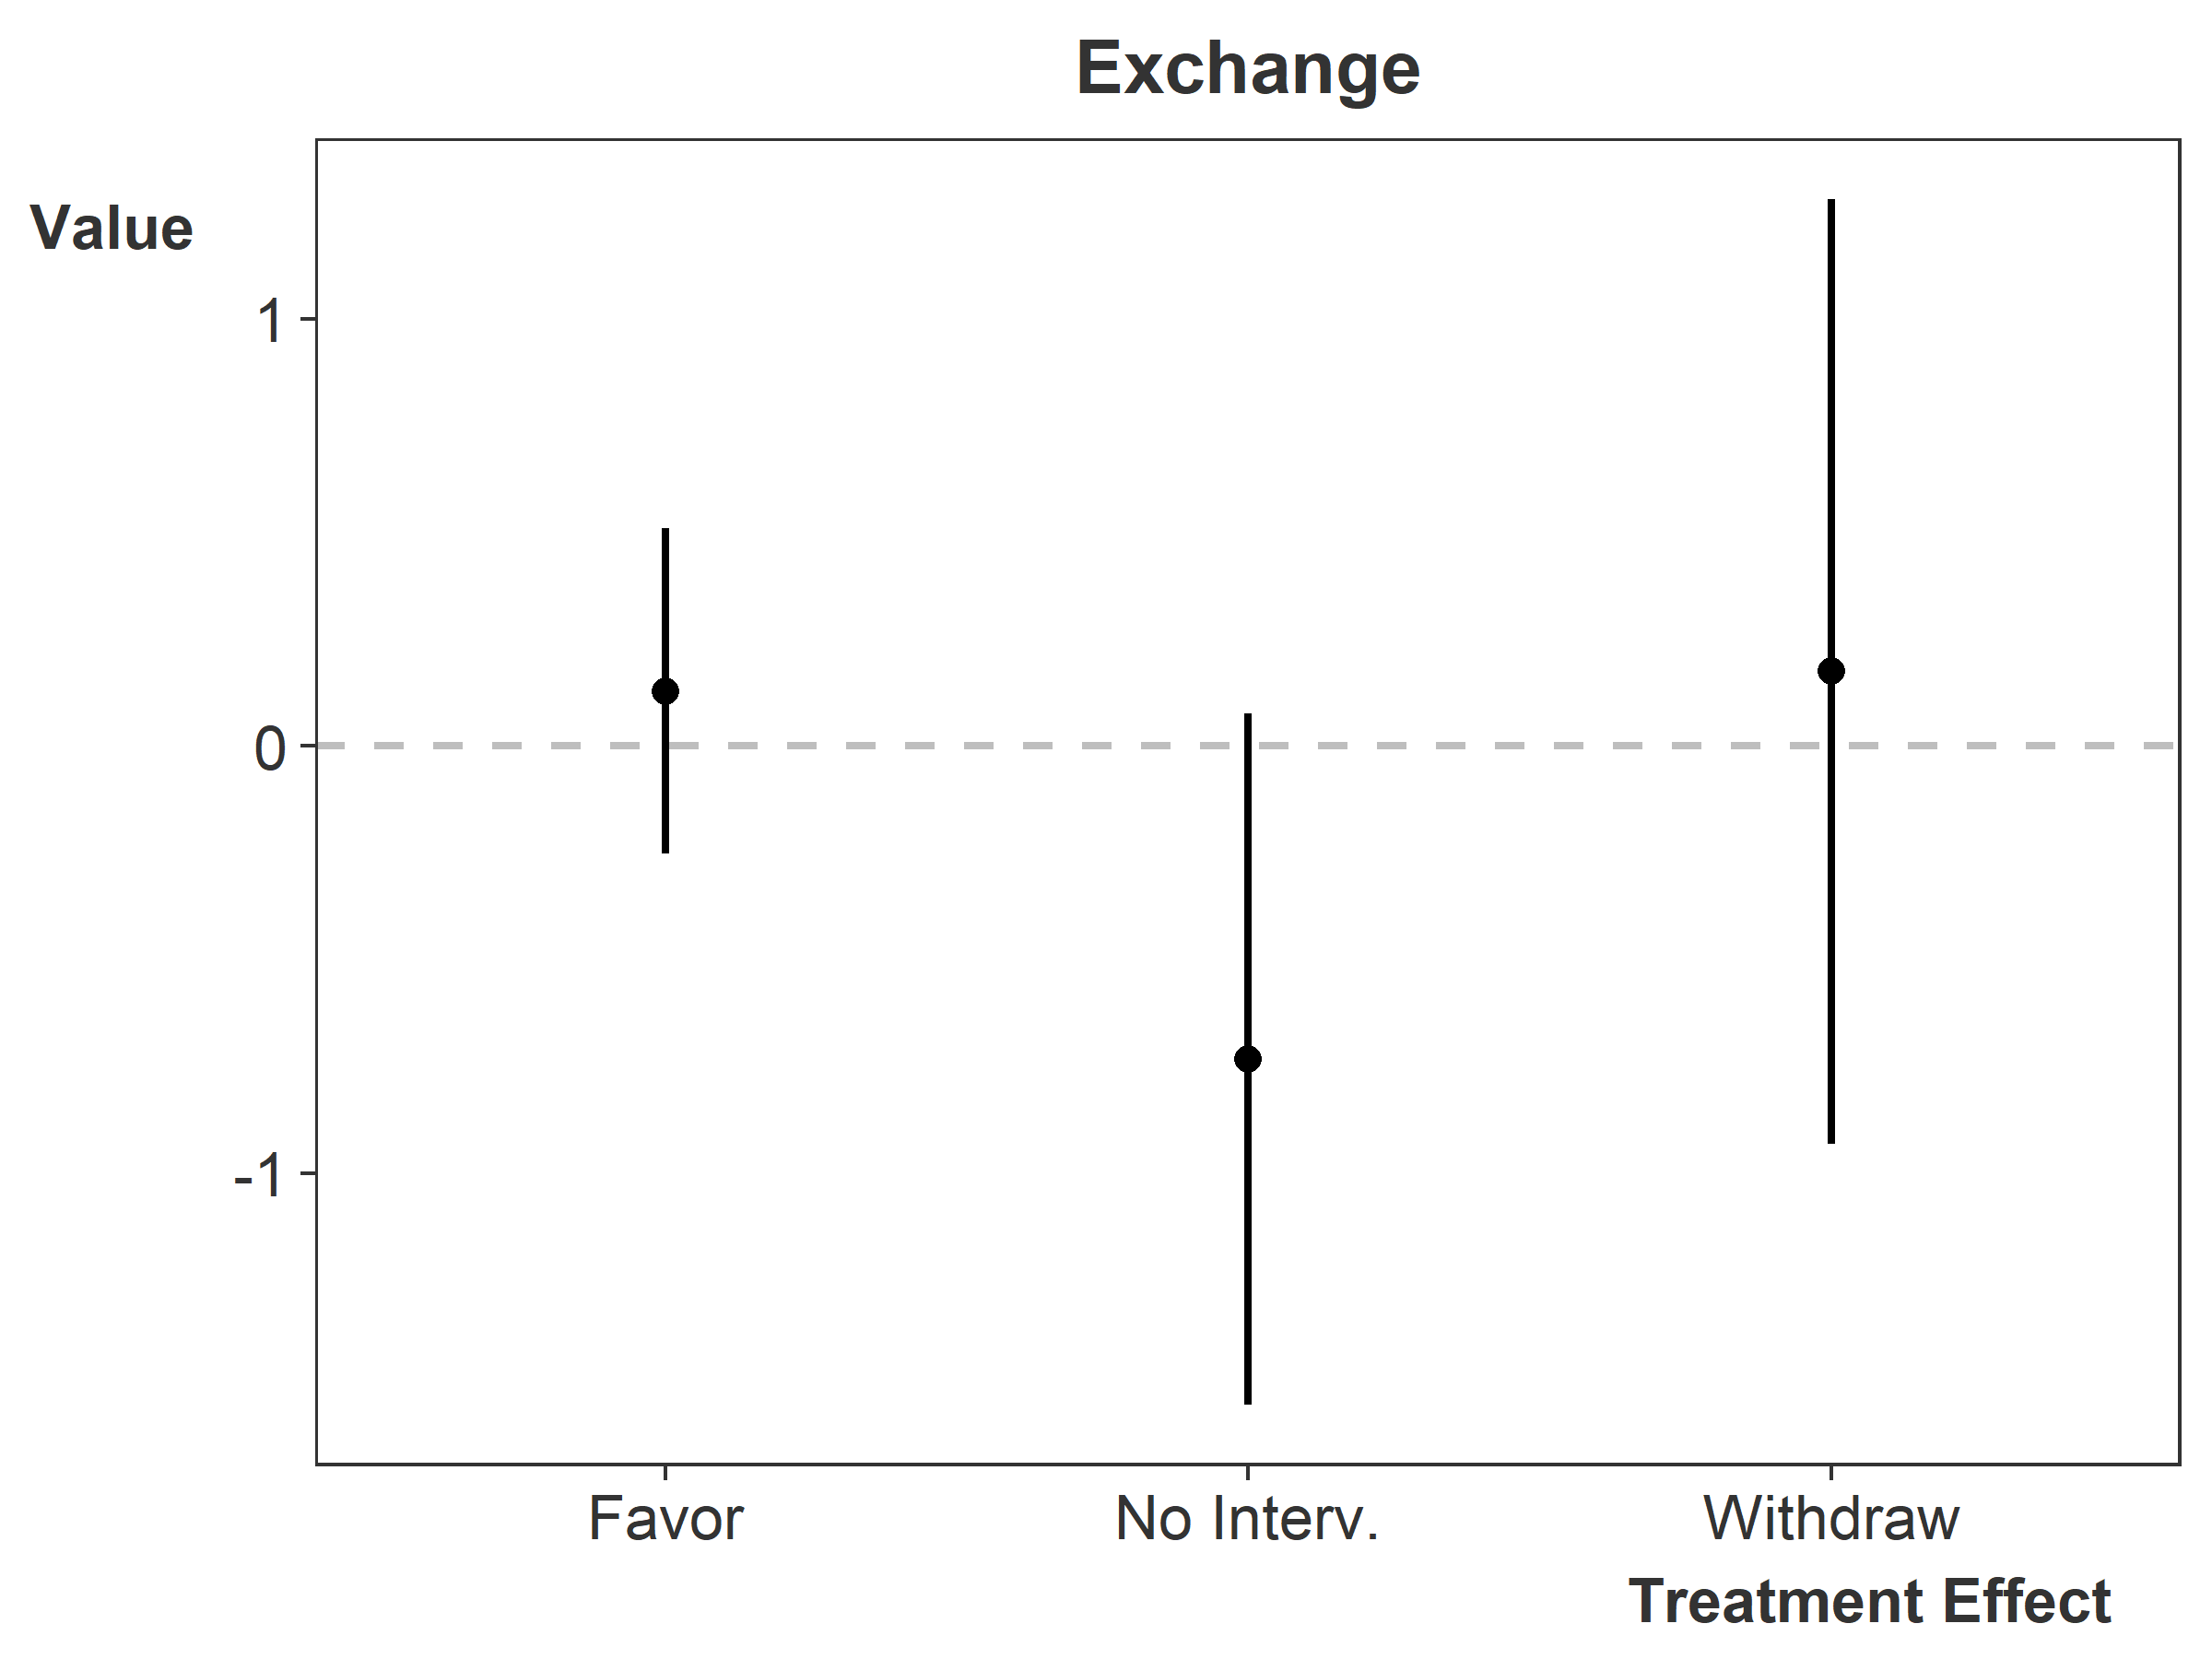
\includegraphics[width=0.95\textwidth]{ex-treat.png}
\end{figure}


\end{frame}


%------------------------------------------------

\begin{frame}{Conclusion}

Mixed evidence at best: would love your thoughts on:

\pause
\begin{enumerate}
\item The argument. 
\pause
\item The experimental design. 
\pause
\item Anything else of note. 
\end{enumerate}


\end{frame}


%-----------------------------------------------

\appendix 

%-----------------------------------------------

\begin{frame}{Demographic Variables/Controls}

\begin{itemize}
\item Partisanship
\item Ideology
\item Foreign Policy Knowledge
\item National Pride 
\item Military Service
\item College Education
\end{itemize} 

\end{frame}


%-----------------------------------------------

\begin{frame}{MTurk Sample Concerns}

\begin{itemize}
\item Lots of Democrats
\item Above-average education
\item Above-average foreign policy knowledge. 
\end{itemize} 

\end{frame}


%-----------------------------------------------


\begin{frame}{Partisanship by Group}

\begin{figure}[htbp]
	\centering
		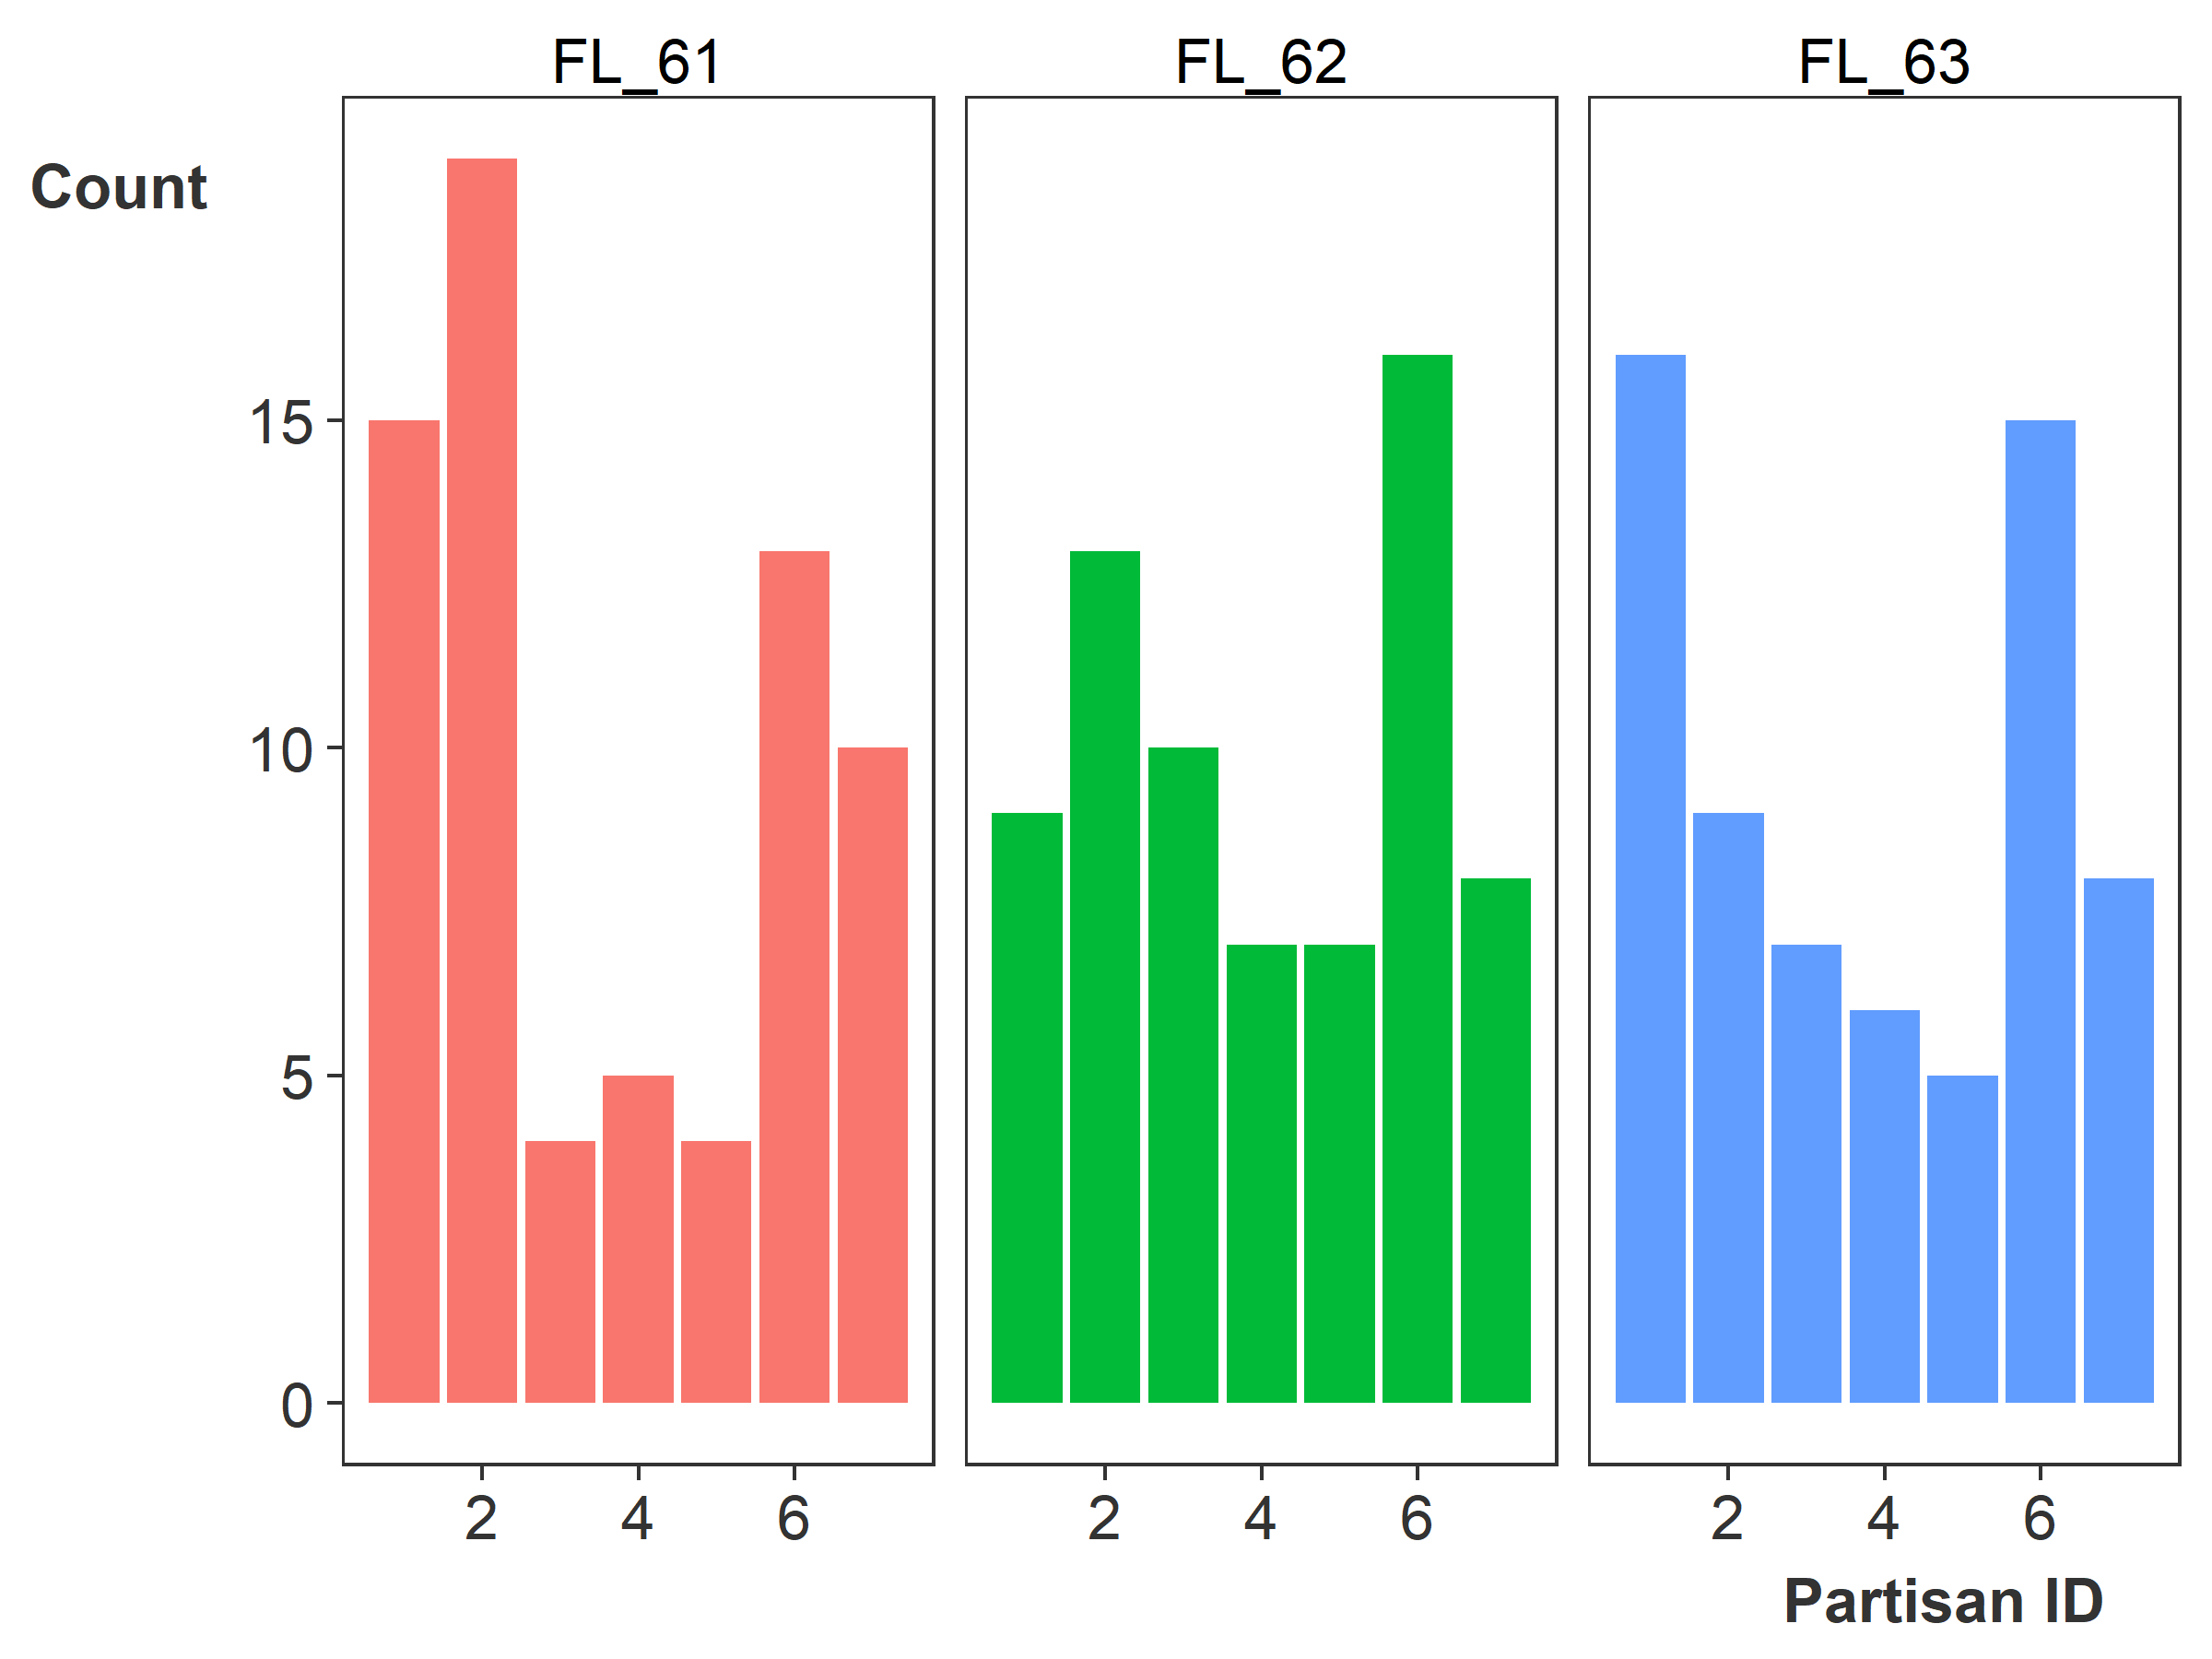
\includegraphics[width=0.95\textwidth]{partisan-group.png}
\end{figure}


\end{frame}

%-----------------------------------------------


\begin{frame}{Mechanism in Neutral Frame}

\begin{figure}[htbp]
	\centering
		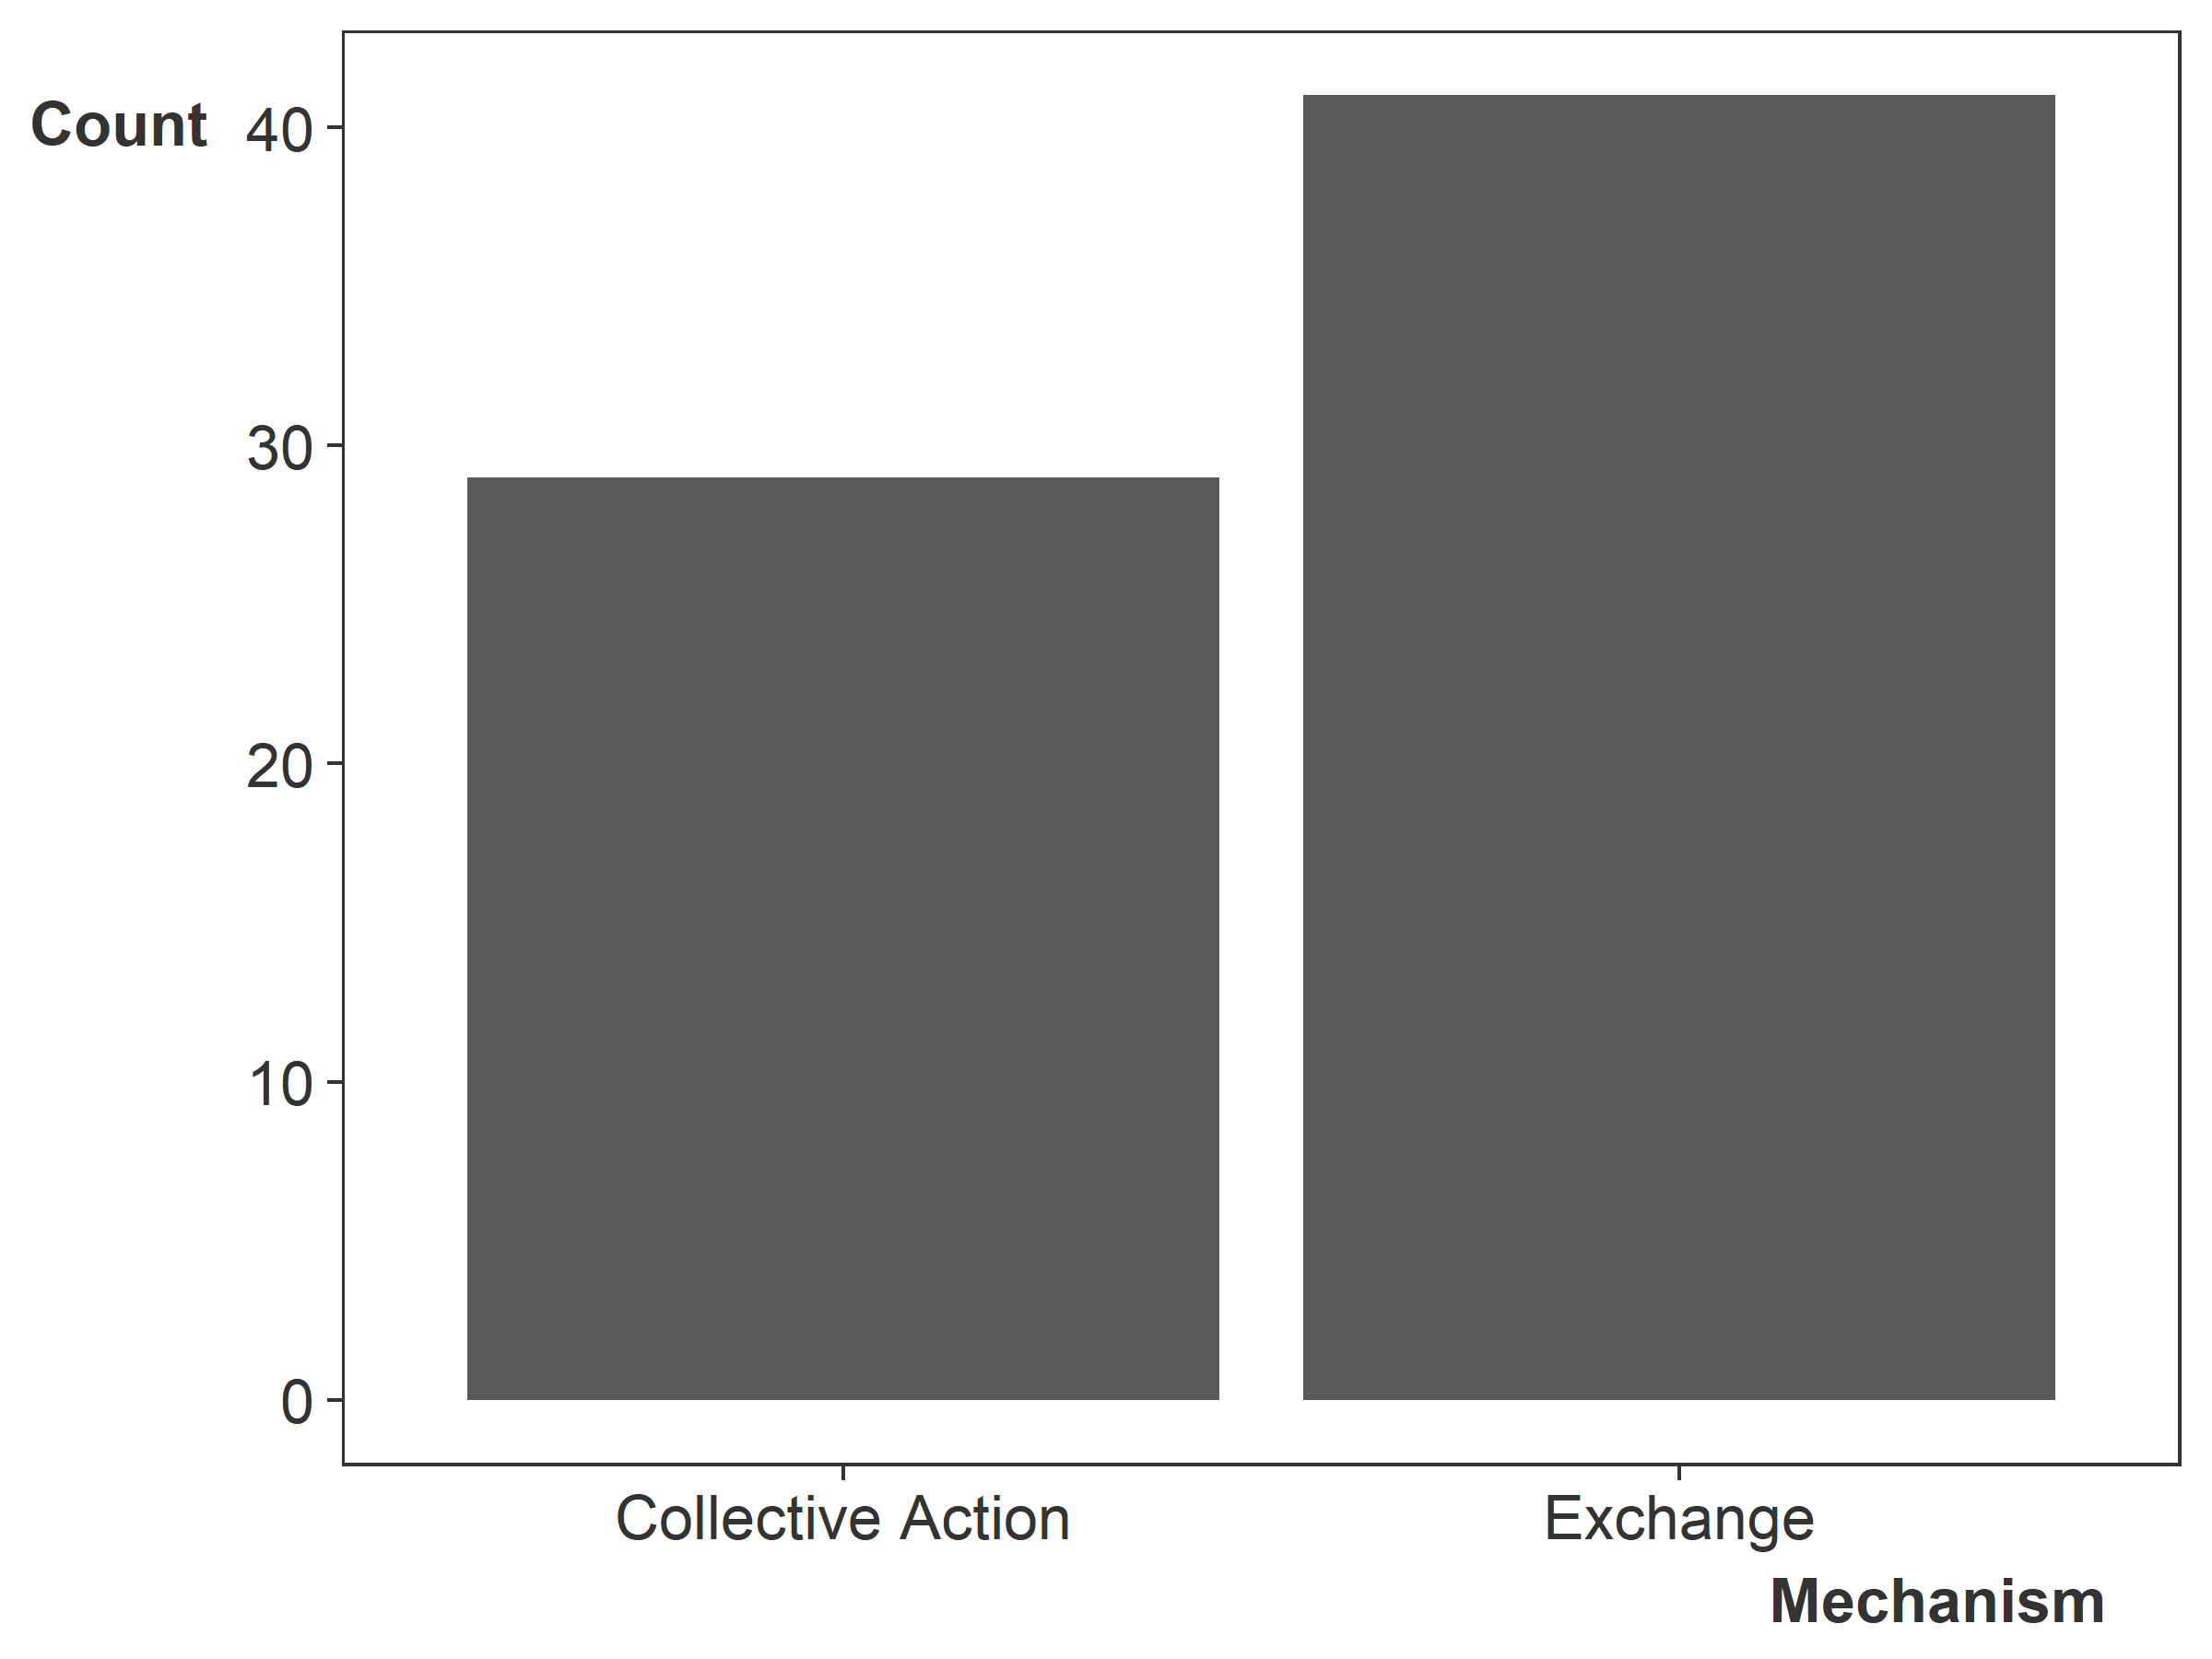
\includegraphics[width=0.95\textwidth]{neutral-mech.png}
\end{figure}


\end{frame}


%--------------------------------------------------

\begin{frame}{Map of Favorability}

\begin{figure}[htbp]
\centering
   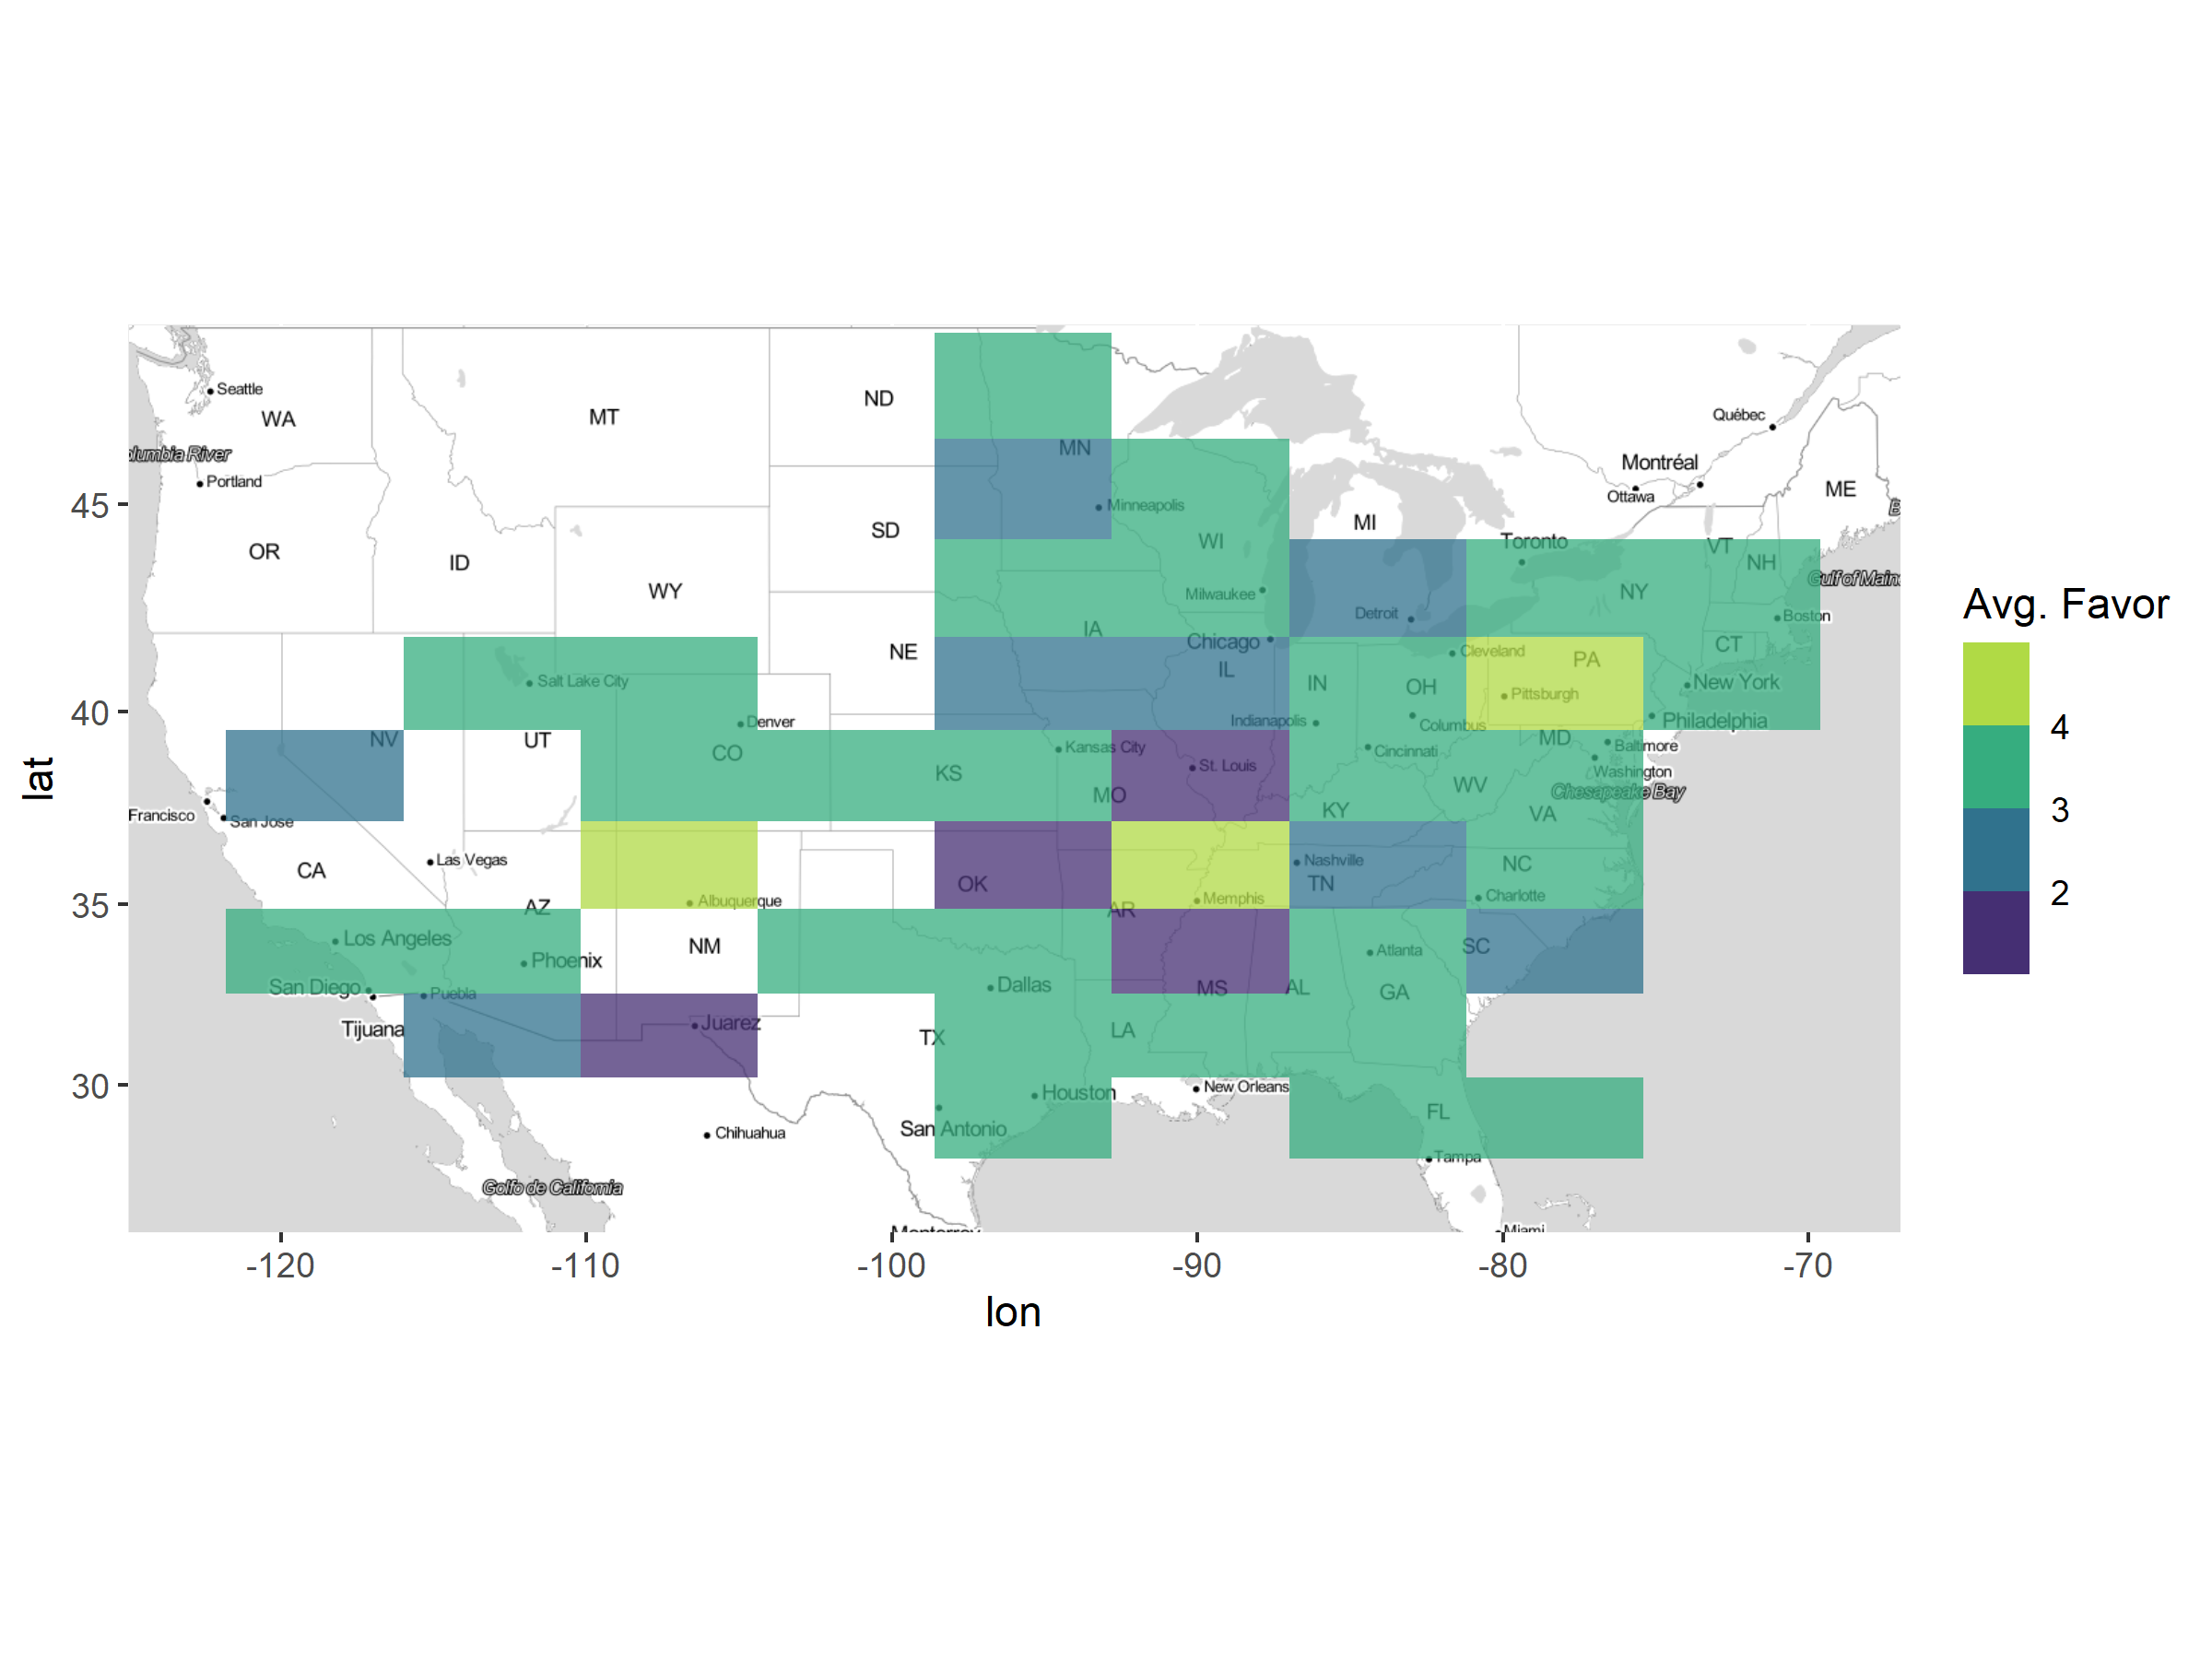
\includegraphics[width=.95\textwidth]{favor-map.png}
\end{figure}

\end{frame}

%---------------------------------------------------

\begin{frame}{Map of Support for Nonintervention} 

\begin{figure}[htbp]
\centering
   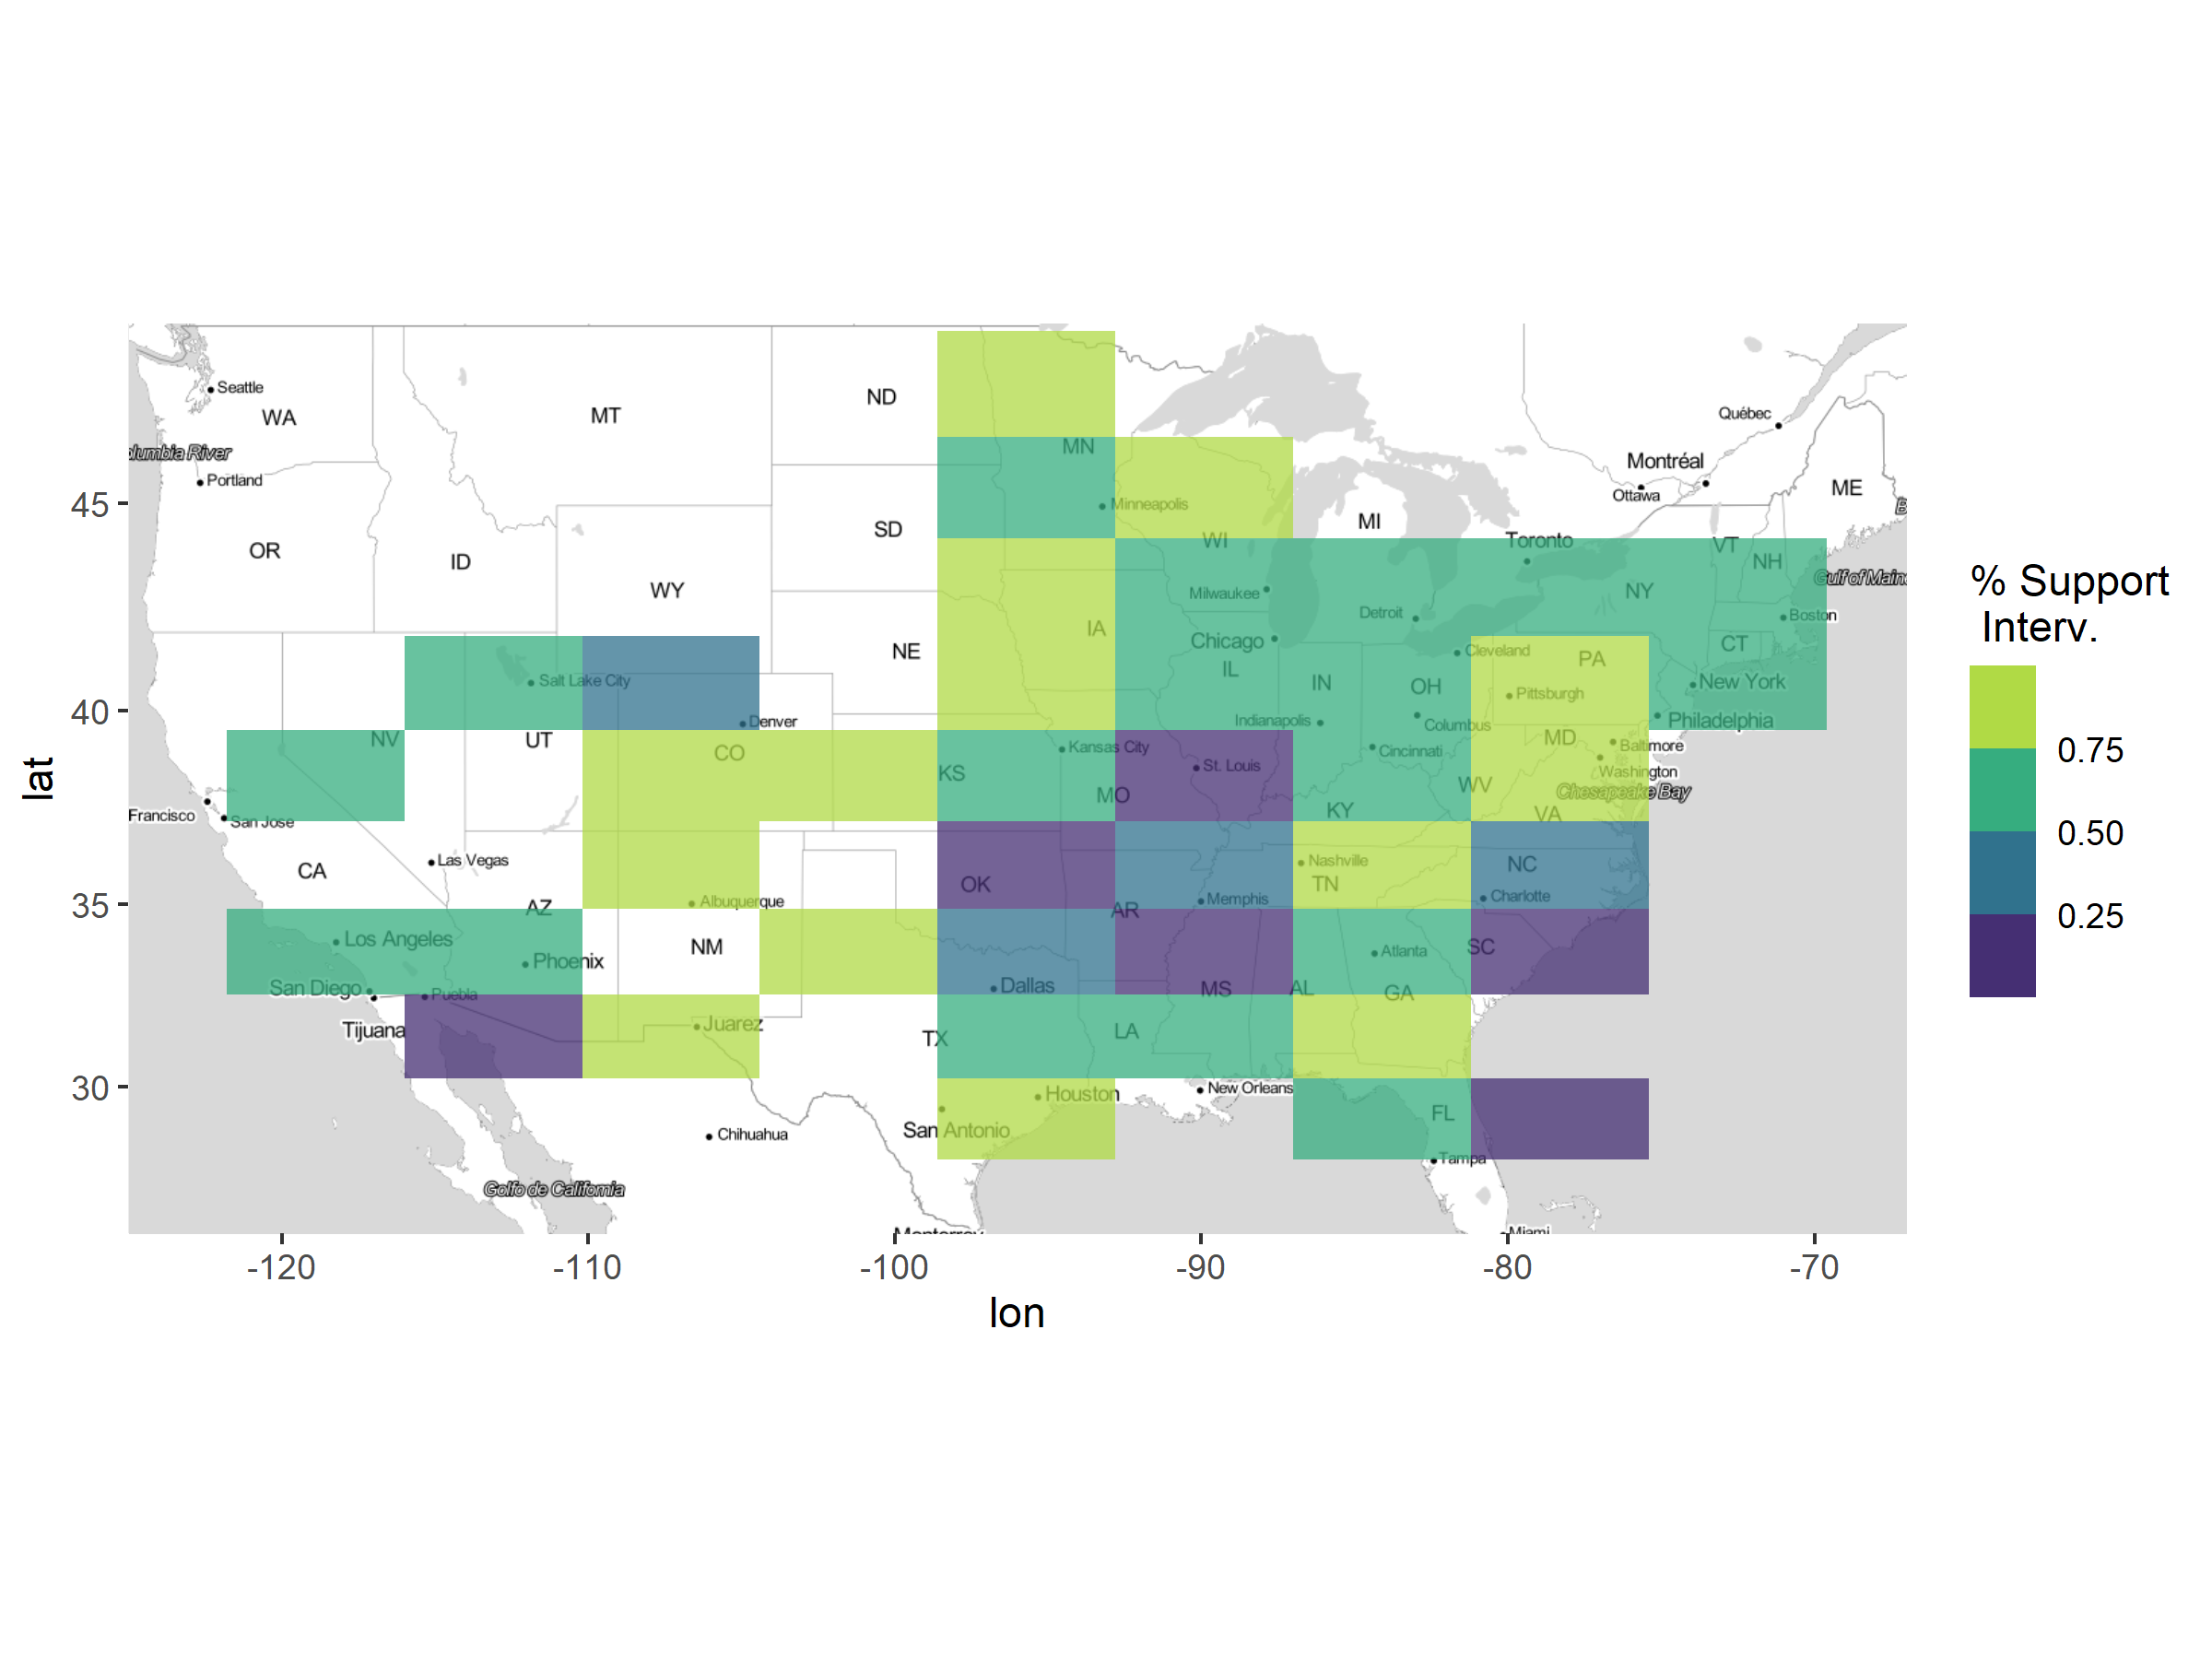
\includegraphics[width = .95\textwidth]{noforce-map.png}
\end{figure}

\end{frame}

%---------------------------------------------------



%----------------------------------------------------------------------------------------

\end{document}
